\documentclass[12pt,a4paper]{report}

% ============================================================
% PACKAGES
% ============================================================
\usepackage[T1]{fontenc}
\usepackage[utf8]{inputenc}
\usepackage[french]{babel}
\usepackage{geometry}
\usepackage{setspace}
\usepackage{graphicx}
\usepackage{titlesec}
\usepackage{tocloft}
\usepackage{array}
\usepackage{longtable}
\usepackage{booktabs}
\usepackage{multirow}
\usepackage{caption}
\usepackage{float}
\usepackage{hyperref}
\usepackage{enumitem}
\usepackage{xcolor}
\usepackage{fancyhdr}
\usepackage{amsmath}
\usepackage{tikz}
\usepackage{ragged2e}
\usepackage{makecell}
\usepackage{tabularx}
\usepackage{microtype}
\usepackage{newtxtext,newtxmath}
\usepackage{listings}
\usetikzlibrary{positioning,arrows.meta}

% ============================================================
% CONFIGURATION GÉNÉRALE
% ============================================================
\geometry{left=2.5cm,right=2.5cm,top=2.5cm,bottom=2.5cm}
\onehalfspacing
\setlength{\parindent}{1.15cm}
\setlength{\parskip}{0.16cm}
\sloppy
\setlength{\emergencystretch}{3em}

\graphicspath{{pics/}{./pics/}{./}}

\definecolor{vinciBlue}{HTML}{1F4FBF}
\definecolor{cegelecRed}{HTML}{D92D27}
\definecolor{reportGray}{HTML}{4A4A4A}
\definecolor{lightGray}{HTML}{F4F6F8}

\newcolumntype{L}[1]{>{\RaggedRight\arraybackslash}p{#1}}
\newcolumntype{Y}{>{\RaggedRight\arraybackslash}X}

\hypersetup{
    colorlinks=true,
    linkcolor=black,
    urlcolor=blue,
    citecolor=black
}

\pagestyle{fancy}
\fancyhf{}
\fancyfoot[R]{\thepage}
\renewcommand{\headrulewidth}{0pt}
\fancypagestyle{plain}{
    \fancyhf{}
    \fancyfoot[R]{\thepage}
    \renewcommand{\headrulewidth}{0pt}
}

\titleformat{\chapter}[display]
  {\bfseries\Large\color{vinciBlue}}
  {\chaptername\ \thechapter}
  {0.5em}
  {\Huge}

\titleformat{\section}
  {\Large\bfseries\color{reportGray}}
  {\thesection}
  {0.8em}
  {}

\titleformat{\subsection}
  {\large\bfseries}
  {\thesubsection}
  {0.8em}
  {}

\titleformat{\subsubsection}
  {\normalsize\bfseries}
  {\thesubsubsection}
  {0.8em}
  {}

% ============================================================
% LISTINGS
% ============================================================
\lstdefinelanguage{json}{
    basicstyle=\ttfamily\small,
    numbers=left,
    numberstyle=\tiny,
    stepnumber=1,
    numbersep=6pt,
    showstringspaces=false,
    breaklines=true,
    frame=single,
    literate=
     *{0}{{{0}}}{1}
      {1}{{{1}}}{1}
      {2}{{{2}}}{1}
      {3}{{{3}}}{1}
      {4}{{{4}}}{1}
      {5}{{{5}}}{1}
      {6}{{{6}}}{1}
      {7}{{{7}}}{1}
      {8}{{{8}}}{1}
      {9}{{{9}}}{1}
      {:}{{{:}}}{1}
      {,}{{{,}}}{1}
      {\{}{{{\{}}}{1}
      {\}}{{{\}}}}{1}
      {[}{{{[}}}{1}
      {]}{{{]}}}{1},
}

\lstdefinelanguage{csharp}{
    basicstyle=\ttfamily\small,
    numbers=left,
    numberstyle=\tiny,
    numbersep=6pt,
    breaklines=true,
    frame=single,
    comment=[l]{//},
    morecomment=[s]{/*}{*/},
    morekeywords={public,private,protected,class,void,string,int,double,bool,var,new,return,foreach,for,while,if,else,using,namespace,static,ref}
}

% ============================================================
% IMAGES ROBUSTES : SI IMAGE MANQUANTE => CADRE À REMPLIR
% ============================================================
\let\realincludegraphics\includegraphics
\renewcommand{\includegraphics}[2][]{%
\IfFileExists{#2}{\realincludegraphics[#1]{#2}}{%
\fbox{\parbox[c][5.0cm][c]{0.92\linewidth}{\centering Image à insérer : \texttt{\detokenize{#2}}}}}%
}

\newcommand{\insertfigure}[3][\textwidth]{%
\begin{figure}[H]
    \centering
    \includegraphics[width=#1]{#2}
    \caption{#3}
\end{figure}}

\newcommand{\figplaceholder}[2]{%
\begin{figure}[H]
    \centering
    \fbox{\parbox[c][5.2cm][c]{0.86\textwidth}{\centering #1}}
    \caption{#2}
\end{figure}}

\newcommand{\importantbox}[1]{%
\begin{center}
\fbox{\begin{minipage}{0.92\textwidth}
#1
\end{minipage}}
\end{center}
}

% ============================================================
\begin{document}
% ============================================================

% ============================================================
% PAGE DE GARDE
% ============================================================
\begin{titlepage}
\newgeometry{left=1.6cm,right=1.6cm,top=1.1cm,bottom=1.1cm}
\thispagestyle{empty}
\centering
\singlespacing
\setlength{\parskip}{0pt}

\noindent
\begin{minipage}[t]{0.25\textwidth}
    \vspace{0pt}
    \centering
    
\includegraphics[width=3.9cm]{pics/ensam.png}
\end{minipage}
\hfill
\begin{minipage}[t]{0.42\textwidth}
    \vspace{35pt}
    \centering
    {\fontsize{12}{14}\selectfont Royaume du Maroc\par}
    \vspace{0.08cm}
    {\fontsize{12}{14}\selectfont Université Mohammed V de Rabat\par}
    \vspace{0.08cm}
    {\fontsize{12}{14}\selectfont École Nationale Supérieure d'Arts et Métiers\par}
\end{minipage}
\hfill
\begin{minipage}[t]{0.25\textwidth}
    \vspace{0pt}
    \centering
    
\includegraphics[width=4cm]{pics/um5_rabat.png}
\end{minipage}

\vspace{1.8cm}

{\fontsize{19}{23}\selectfont\bfseries RAPPORT DE PROJET DE FIN D'ÉTUDES\par}

\vspace{0.55cm}

{\fontsize{12}{15}\selectfont Présenté pour obtenir le titre de :\par}
\vspace{0.15cm}
{\fontsize{17}{21}\selectfont\bfseries INGÉNIEUR D'ÉTAT\par}
\vspace{0.10cm}
{\fontsize{12}{15}\selectfont\bfseries EN\par}
\vspace{0.10cm}
{\fontsize{15}{19}\selectfont\bfseries Énergie Électrique et Industrie Numérique\par}

\vspace{0.45cm}
{\color{cegelecRed}\rule{0.17\textwidth}{0.9pt}\par}
\vspace{0.50cm}

{\fontsize{17}{23}\selectfont\bfseries
Développement d'une solution BIM intelligente\\[0.16cm]
pour l'automatisation des réservations structurelles\\[0.16cm]
et l'intégration BIM--IoT appliquée à la\\[0.16cm]
supervision technique des bâtiments\par}

\vspace{0.55cm}

{\fontsize{12}{15}\selectfont Société d'accueil : \textbf{VINCI Energies Building Solutions}\par}
\vspace{0.18cm}

\includegraphics[width=7cm]{pics/entreprise_vinci_building_solutions.png}

\vspace{0.55cm}

{\fontsize{12}{15}\selectfont\bfseries Réalisé par :\par}
\vspace{0.10cm}
{\fontsize{17}{21}\selectfont\bfseries Badr AZIZI\par}

\vspace{0.50cm}

{\fontsize{12}{15}\selectfont\bfseries Encadré par :\par}
\vspace{0.20cm}

\begin{tabular}{@{}p{5.2cm}p{10.5cm}@{}}
\textbf{M. ATMAN JBARI} &
Encadrant académique, ENSAM Rabat \\[0.18cm]
\textbf{Mme Nouhaila LAFDIL} &
Encadrante industrielle, VINCI Energies Building Solutions \\
\end{tabular}

\vspace{0.30cm}

{\fontsize{12}{15}\selectfont\bfseries Soutenu le 15/06/2026 devant le jury :\par}

\vspace{0.22cm}

\begin{tabular}{@{}p{5.2cm}p{10.5cm}@{}}
\textbf{M. ATMAN JBARI} & Encadrant académique \\[0.14cm]
\textbf{Mme Nouhaila LAFDIL} & Encadrante industrielle \\[0.14cm]
\textbf{M. Nom du président du jury} & Président du jury \\[0.14cm]
\textbf{M. Nom du rapporteur} & Rapporteur \\
\end{tabular}

\vfill

{\fontsize{12}{15}\selectfont\bfseries Année universitaire : 2025--2026\par}

\restoregeometry
\end{titlepage}

% ============================================================
% PAGES LIMINAIRES
% ============================================================
\pagenumbering{Roman}

\chapter*{Avant-propos}
\addcontentsline{toc}{chapter}{Avant-propos}
\begin{longtable}{>{\bfseries}p{5.0cm}p{9.5cm}}
Nom et prénom du stagiaire : & Badr AZIZI \\
Intitulé du travail : & Développement d'une solution BIM intelligente pour l'automatisation des réservations structurelles et l'intégration BIM--IoT appliquée à la supervision technique des bâtiments \\
Entreprise d'accueil : & VINCI Energies Building Solutions \\
Entité d'accueil : & Cellule BIM / BIM\&SYN -- BE Fluides, BIM et Synthèse \\
Établissement : & École Nationale Supérieure d'Arts et Métiers de Rabat \\
Période du PFE : & Année universitaire 2025--2026 \\
\end{longtable}

\chapter*{Dédicace}
\addcontentsline{toc}{chapter}{Dédicace}
Rédiger la dédicace finale.

\chapter*{Remerciements}
\addcontentsline{toc}{chapter}{Remerciements}
Rédiger les remerciements personnalisés avec les noms définitifs.

\chapter*{Résumé}
\addcontentsline{toc}{chapter}{Résumé}
Ce mémoire présente les travaux réalisés dans le cadre d'un projet de fin d'études au sein de VINCI Energies Building Solutions. Le travail s'articule autour de trois contributions complémentaires : la participation à la modélisation BIM du projet C2R, le développement d'un plugin Revit nommé RESBIM pour l'automatisation du traitement des réservations structurelles, et la mise en œuvre d'une intégration BIM--IoT basée sur ESP32, MQTT, Node-RED et Revit pour la supervision technique des bâtiments.

Le besoin principal identifié concerne le traitement des réservations structurelles dans les projets BIM multidisciplinaires. Le processus classique repose sur la détection des conflits, l'analyse manuelle, la création des réservations dans Revit, puis leur vérification et leur suivi. Ce workflow devient rapidement chronophage lorsque le nombre de traversées MEP augmente et peut générer des erreurs de dimensions, de niveaux, de support, de statut ou de traçabilité.

La solution RESBIM vise à automatiser la détection, la génération, le dimensionnement, le placement, l'orientation, la fusion, la vérification, la numérotation, la visualisation et l'échange des données des réservations. La partie BIM--IoT complète cette démarche en reliant des données issues d'un ESP32 à des objets Revit afin de visualiser l'état technique des équipements dans la maquette numérique.

\textbf{Mots-clés :} BIM, Revit, RESBIM, réservations structurelles, coordination MEP--Structure, C\#, Dynamo, ESP32, MQTT, Node-RED, BIM--IoT, supervision technique.

\chapter*{Abstract}
\addcontentsline{toc}{chapter}{Abstract}
This final-year project presents the work carried out at VINCI Energies Building Solutions. The project is structured around three complementary contributions: participation in the BIM modelling of the C2R project, the development of a Revit plugin named RESBIM for the automation of structural openings, and the implementation of a BIM--IoT integration based on ESP32, MQTT, Node-RED and Revit for technical building supervision.

The main identified need concerns the handling of structural openings in multidisciplinary BIM projects. The conventional workflow relies on clash detection, manual analysis, reservation creation in Revit, and follow-up through views, parameters and schedules. This process becomes time-consuming and may lead to errors in dimensions, levels, host elements, status and traceability.

RESBIM aims to automate detection, generation, sizing, placement, orientation, merging, verification, numbering, visualization and data exchange related to structural reservations. The BIM--IoT part extends this approach by linking ESP32 data to Revit objects in order to visualize technical equipment states directly in the digital model.

\textbf{Keywords:} BIM, Revit, RESBIM, structural openings, MEP--Structure coordination, C\#, Dynamo, ESP32, MQTT, Node-RED, BIM--IoT, technical supervision.

\chapter*{Liste des abréviations}
\addcontentsline{toc}{chapter}{Liste des abréviations}
\begin{longtable}{>{\bfseries}p{3cm}p{10.5cm}}
BIM & Building Information Modeling \\
MEP & Mechanical, Electrical and Plumbing \\
CFO & Courant Fort \\
CFA & Courant Faible \\
CVC & Chauffage, Ventilation et Climatisation \\
API & Application Programming Interface \\
IoT & Internet of Things \\
MQTT & Message Queuing Telemetry Transport \\
XML & eXtensible Markup Language \\
UI & User Interface \\
KPI & Key Performance Indicator \\
ESP32 & Microcontrôleur Wi-Fi/Bluetooth utilisé pour la communication IoT \\
\end{longtable}

\tableofcontents
\listoffigures
\listoftables

\clearpage
\pagenumbering{arabic}

% ============================================================
% INTRODUCTION GÉNÉRALE
% ============================================================
\chapter*{Introduction générale}
\addcontentsline{toc}{chapter}{Introduction générale}

\section*{Contexte général}
\addcontentsline{toc}{section}{Contexte général}
Les projets de bâtiment deviennent de plus en plus complexes en raison de la multiplication des disciplines techniques, de la réduction des délais d'exécution et de l'augmentation des exigences de qualité. Dans ce contexte, le Building Information Modeling constitue un support essentiel pour la modélisation, la coordination, la synthèse et la gestion de l'information entre les intervenants.

Au sein de VINCI Energies Building Solutions, la cellule BIM \& Synthèse intervient dans un environnement où les maquettes architecture, structure, fluides, CFO, CFA et synthèse doivent être coordonnées afin de limiter les conflits avant l'exécution. Les réseaux techniques traversent fréquemment les voiles et les dalles, ce qui nécessite la création de réservations structurelles correctement dimensionnées, positionnées, vérifiées et traçables.

\section*{Positionnement du PFE}
\addcontentsline{toc}{section}{Positionnement du PFE}
Le présent PFE s'inscrit dans une démarche de digitalisation et d'automatisation des méthodes BIM. Il regroupe trois axes complémentaires mais clairement séparés :
\begin{enumerate}[leftmargin=1.2cm]
    \item la contribution à la modélisation BIM du projet C2R ;
    \item le développement de RESBIM, un plugin Revit dédié à l'automatisation des réservations structurelles ;
    \item l'intégration BIM--IoT avec ESP32 pour la supervision technique d'équipements dans la maquette.
\end{enumerate}

Cette organisation permet de distinguer le travail de production BIM, le travail de développement logiciel et le travail d'intégration IoT, tout en montrant leur cohérence dans une même démarche numérique.

\section*{Objectifs du projet}
\addcontentsline{toc}{section}{Objectifs du projet}
Les objectifs principaux du PFE sont :
\begin{itemize}[leftmargin=1.2cm]
    \item participer à la modélisation BIM du projet C2R, notamment les maquettes architecture, structure, fluides, CFO, CFA et synthèse ;
    \item analyser le besoin métier lié au traitement des réservations structurelles ;
    \item concevoir et développer le plugin RESBIM sous Revit ;
    \item automatiser la génération, le dimensionnement, la vérification et le suivi des réservations ;
    \item intégrer une chaîne BIM--IoT basée sur ESP32, MQTT, Node-RED et Revit ;
    \item mesurer la valeur ajoutée du travail à travers des cas tests, des résultats Excel et une comparaison avant/après.
\end{itemize}

\section*{Démarche adoptée}
\addcontentsline{toc}{section}{Démarche adoptée}
La démarche suivie commence par la compréhension du contexte industriel et la formulation de la problématique. Elle se poursuit par une étude des concepts techniques nécessaires, puis par la contribution à la modélisation BIM du projet C2R. La phase suivante concerne la conception et le développement de RESBIM, en intégrant une phase de prototypage sous Dynamo, la préparation des familles et des paramètres, puis la migration vers une solution C\# plus robuste. Enfin, une couche BIM--IoT est mise en œuvre à travers ESP32, MQTT, Node-RED et Revit, avant de présenter les validations, les résultats et les perspectives.

\section*{Organisation du rapport}
\addcontentsline{toc}{section}{Organisation du rapport}
Le rapport est structuré en sept chapitres. Le premier présente l'organisme d'accueil et le cadre général du projet. Le deuxième formalise la problématique et l'analyse du besoin. Le troisième expose l'état de l'art nécessaire à la compréhension du sujet. Le quatrième présente la contribution à la modélisation BIM du projet C2R. Le cinquième est consacré à la conception et au développement de RESBIM. Le sixième détaille l'intégration BIM--IoT avec ESP32. Le septième présente la validation, les résultats, la valeur ajoutée et la participation au challenge d'innovation VEAO VINCI.

% ===========================
% CHAPITRE 1
% ===========================
\chapter{Organisme d'accueil et cadre général du projet}

\section{Introduction}

Ce chapitre présente le cadre industriel dans lequel s'inscrit le projet de fin d'études. Il présente d'abord le groupe VINCI et sa branche VINCI Energies, puis l'entité d'accueil VINCI Energies Building Solutions Maroc. Il précise ensuite le rôle de la cellule BIM \& Synthèse, qui constitue l'environnement direct du PFE, ainsi que les missions confiées durant le stage.

L'objectif de ce chapitre est de situer le projet dans son contexte professionnel afin de montrer la cohérence entre les besoins de l'entreprise, les enjeux de coordination BIM et le développement d'une solution d'automatisation nommée RESBIM.

% ------------------------------------------------------------
\section{Présentation de VINCI Energies}

VINCI Energies est une branche du groupe VINCI spécialisée dans les métiers de l'énergie, des infrastructures, de l'industrie, des technologies de l'information et du bâtiment. Elle accompagne ses clients dans la conception, la réalisation, l'intégration, l'exploitation et la maintenance de systèmes techniques complexes.

Dans le contexte actuel de transformation numérique et de transition énergétique, VINCI Energies développe des solutions visant à améliorer la performance des bâtiments, la fiabilité des installations, la qualité d'exécution et l'exploitation des données techniques. Cette orientation rend l'utilisation du BIM particulièrement importante, car la maquette numérique devient un support de coordination, de contrôle et d'aide à la décision.

\begin{figure}[H]
    \centering
    
\includegraphics[width=0.50\textwidth]{pics/entreprise_vinci_building_solutions.png}
    \caption{VINCI Energies -- Building Solutions}
\end{figure}

\subsection{Implantation internationale et présence au Maroc}

VINCI Energies dispose d'une présence internationale importante. Cette implantation permet au groupe d'intervenir sur des projets variés, allant des infrastructures énergétiques aux bâtiments techniques, en passant par l'industrie, les réseaux de communication et les solutions numériques.

Au Maroc, VINCI Energies intervient à travers plusieurs entités spécialisées. Cette présence locale permet de répondre aux besoins des projets nationaux tout en bénéficiant des méthodes, standards et retours d'expérience du groupe.

\begin{figure}[H]
    \centering
    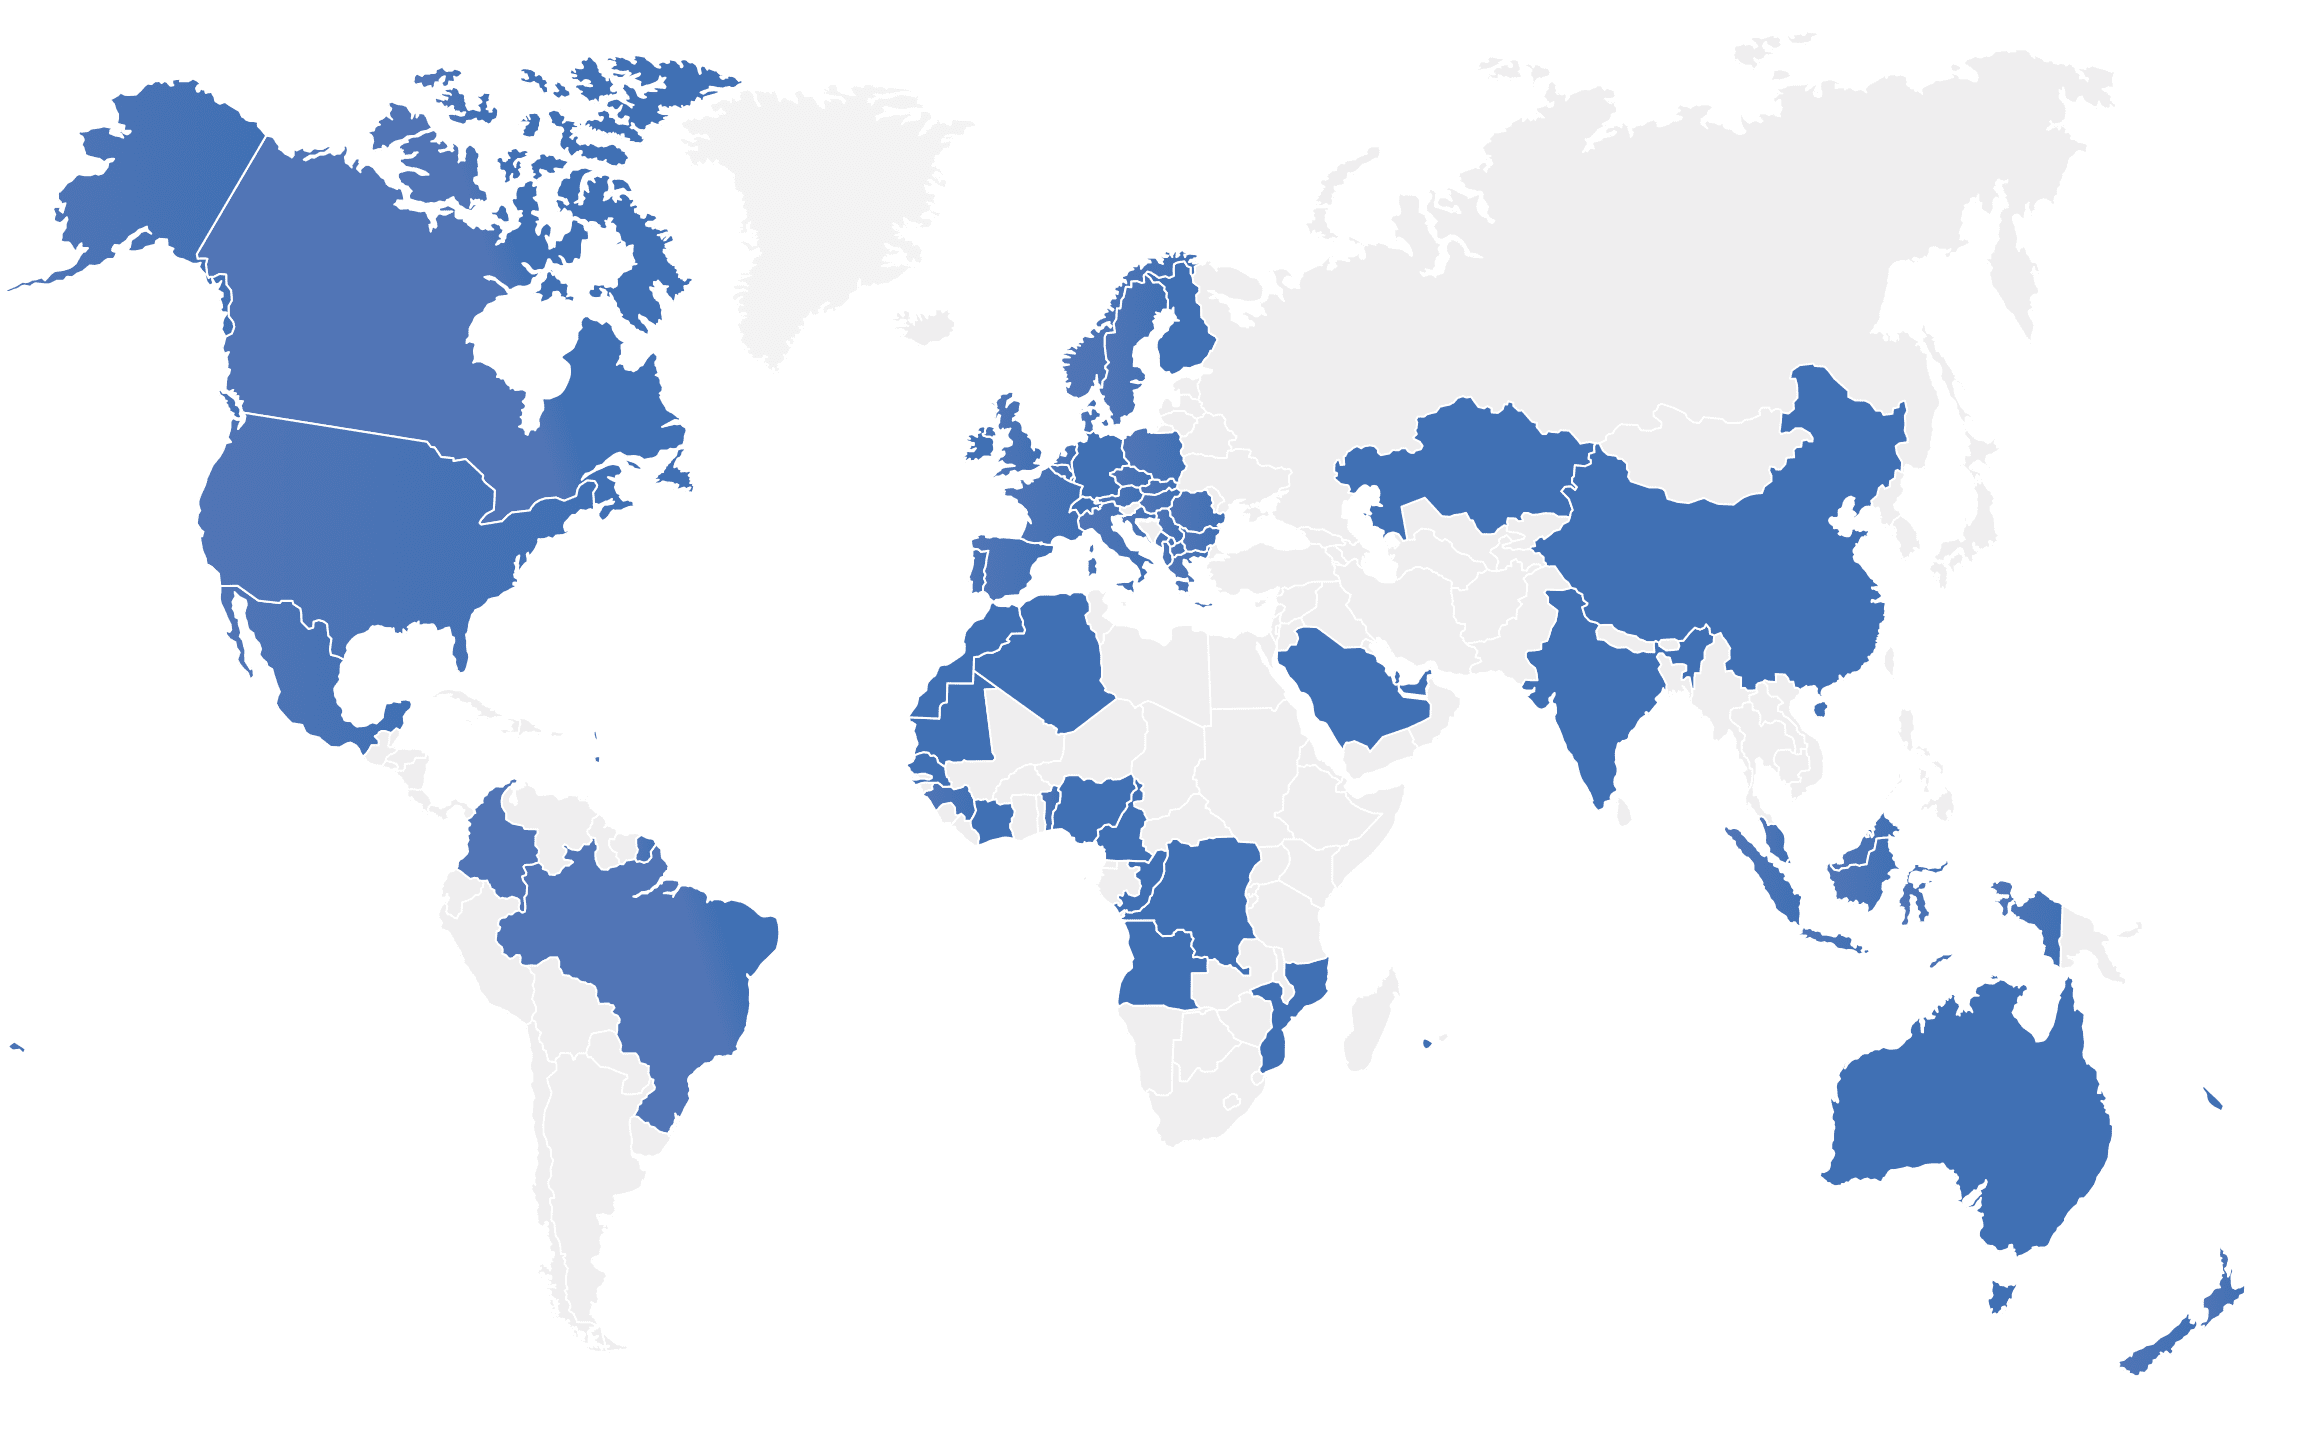
\includegraphics[width=0.88\textwidth]{pics/implantation_monde_vinci_energies.png}
    \caption{Implantation de VINCI Energies dans le monde}
\end{figure}

\begin{figure}[H]
    \centering
    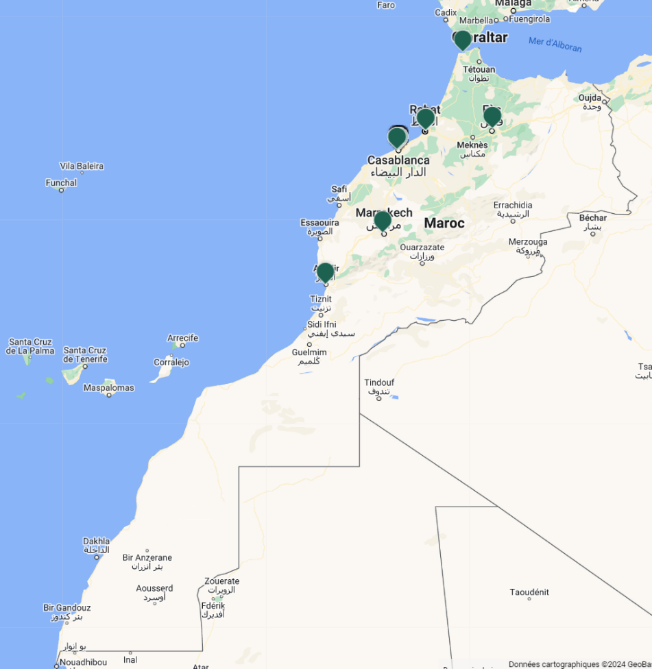
\includegraphics[width=0.78\textwidth]{pics/implantation_maroc_vinci_energies.png}
    \caption{Implantation de VINCI Energies au Maroc}
\end{figure}

\subsection{Domaines d'activité}

Les activités de VINCI Energies couvrent plusieurs domaines complémentaires : énergie, bâtiment, industrie, infrastructures, technologies de l'information, automatisation, sûreté et maintenance. Dans les projets de bâtiment, cette diversité implique une forte coordination entre les lots techniques, notamment les réseaux électriques, les fluides, le CVC, la plomberie, la sécurité incendie et les systèmes de communication.

Cette diversité explique l'importance d'une démarche BIM structurée. En effet, la coordination des maquettes architecture, structure, fluides, CFO et CFA permet d'anticiper les conflits, de fiabiliser les livrables et de réduire les reprises en phase d'exécution.

\begin{figure}[H]
    \centering
    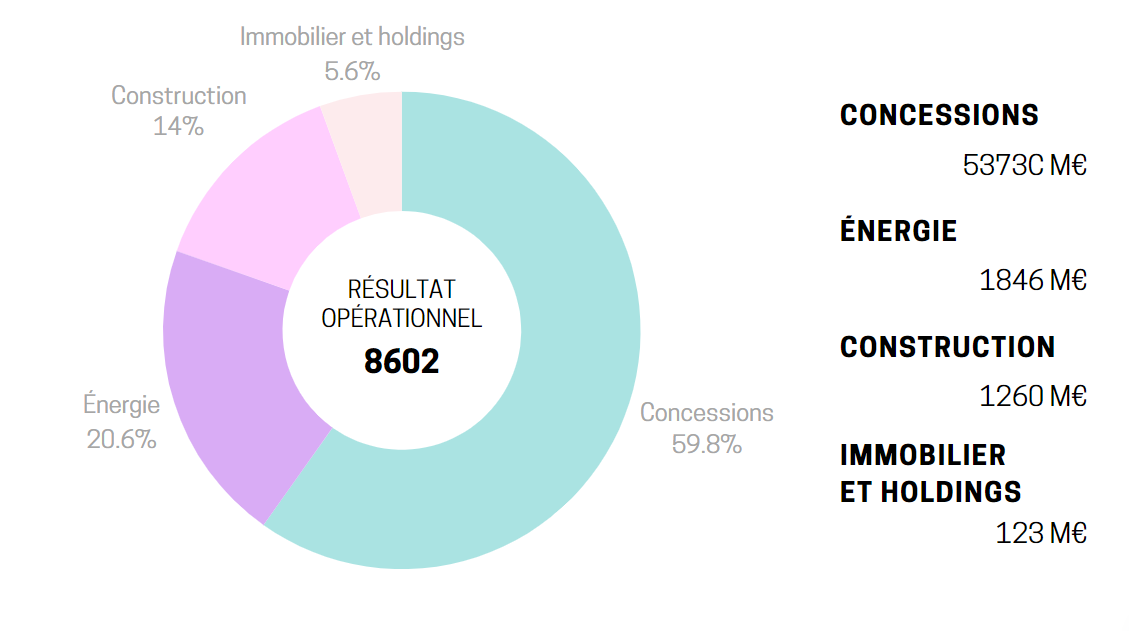
\includegraphics[width=0.86\textwidth]{pics/activites_vinci.png}
    \caption{Principales activités de VINCI Energies}
\end{figure}

\begin{figure}[H]
    \centering
    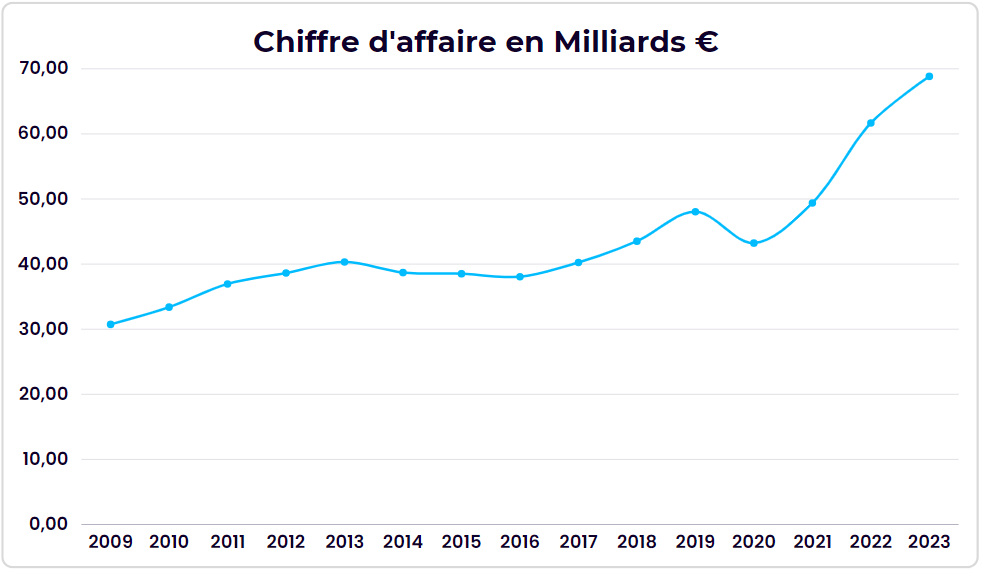
\includegraphics[width=0.86\textwidth]{pics/chiffre_affaires_vinci.png}
    \caption{Indicateurs économiques et chiffre d'affaires du groupe}
\end{figure}

% ------------------------------------------------------------
\section{Présentation de VINCI Energies Building Solutions Maroc}

VINCI Energies Building Solutions Maroc constitue l'entité d'accueil du présent projet de fin d'études. Elle intervient dans la conception, la réalisation et l'intégration des lots techniques dans les bâtiments et infrastructures. Ses domaines d'intervention couvrent notamment les installations électriques, les courants forts, les courants faibles, les fluides, le CVC, la plomberie, la sûreté, la sécurité incendie, les systèmes de contrôle et la synthèse technique.

Dans ce type d'environnement, la coordination entre les disciplines est essentielle. Les réseaux techniques doivent cohabiter avec la structure et l'architecture, ce qui impose une organisation rigoureuse des maquettes, des vues de contrôle et des échanges entre intervenants. C'est dans ce cadre que s'inscrit le besoin d'automatiser certaines tâches répétitives, notamment le traitement des réservations structurelles.

\begin{figure}[H]
    \centering
    
\includegraphics[width=0.58\textwidth]{pics/entreprise_vinci_building_solutions.png}
    \caption{Positionnement de l'entité d'accueil dans VINCI Energies Building Solutions}
\end{figure}

% ------------------------------------------------------------
\section{Engagement qualité, sécurité et environnement}

Les projets réalisés par VINCI Energies Building Solutions s'inscrivent dans une démarche qualité, sécurité et environnement. Cette démarche vise à assurer la conformité des livrables, la maîtrise des risques, la sécurité des équipes et la fiabilité des installations techniques.

Dans le cadre du BIM, cette exigence se traduit par la nécessité de produire des maquettes propres, structurées, coordonnées et exploitables. Les objets BIM doivent être correctement renseignés, les vues doivent être lisibles, et les informations doivent être traçables. Ces exigences sont directement liées au développement de RESBIM, dont l'objectif est de fiabiliser le traitement des réservations et d'améliorer la qualité du processus de coordination.

\begin{figure}[H]
    \centering
    
\includegraphics[width=0.58\textwidth]{pics/charte_qse_cegelec.png}
    \caption{Charte qualité, sécurité et environnement de l'entité d'accueil}
\end{figure}

\begin{figure}[H]
    \centering
    \begin{minipage}[c]{0.30\textwidth}
        \centering
        
\includegraphics[width=0.88\linewidth]{pics/certification_iso_9001.png}
    \end{minipage}
    \hfill
    \begin{minipage}[c]{0.30\textwidth}
        \centering
        
\includegraphics[width=0.88\linewidth]{pics/certification_iso_14001.png}
    \end{minipage}
    \hfill
    \begin{minipage}[c]{0.30\textwidth}
        \centering
        
\includegraphics[width=0.88\linewidth]{pics/certification_iso_45001.png}
    \end{minipage}
    \caption{Certifications qualité, environnement, santé et sécurité}
\end{figure}

% ------------------------------------------------------------
\section{Organisation de VINCI Energies et positionnement de la cellule BIM}

L'organisation de VINCI Energies repose sur des entités opérationnelles spécialisées, capables de répondre à des besoins techniques variés. Cette organisation favorise la proximité avec les projets et l'adaptation aux contraintes locales.

Dans ce cadre, la cellule BIM \& Synthèse occupe un rôle transversal. Elle intervient comme support de coordination entre les disciplines et contribue à l'amélioration des méthodes numériques. Elle participe à la production des maquettes, à la gestion des liens, à la préparation des vues de synthèse, à la détection des conflits et à la fiabilisation des livrables BIM.

\begin{figure}[H]
    \centering
    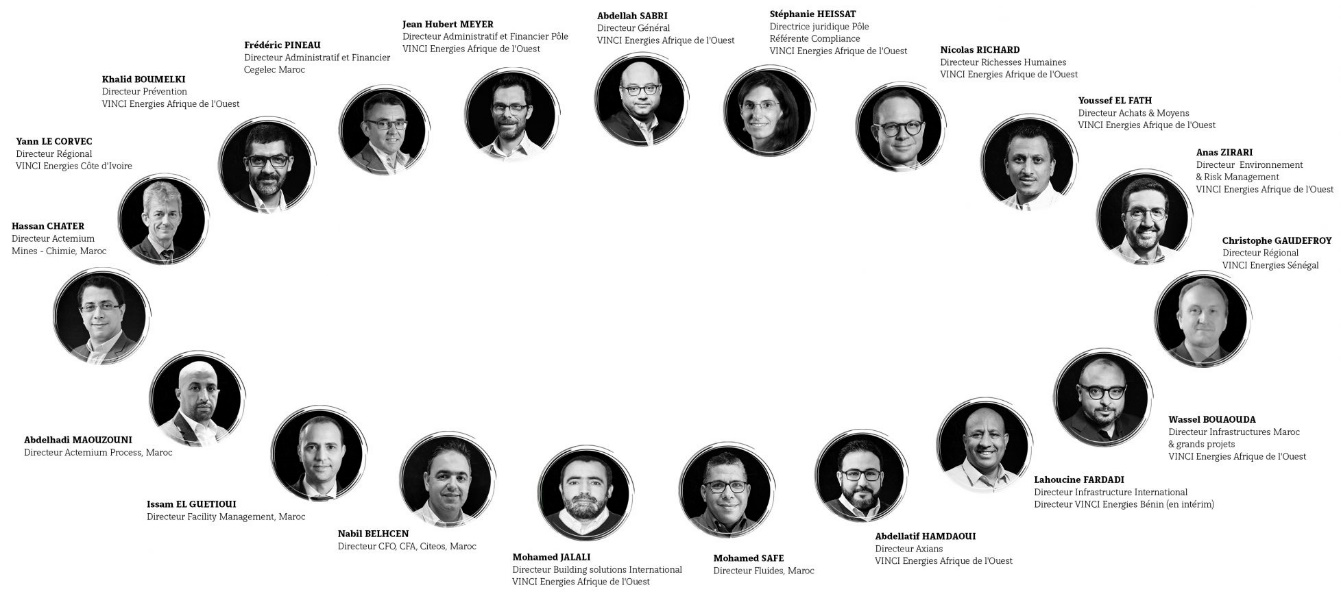
\includegraphics[width=0.84\textwidth]{pics/organigramme_vinci_energies.png}
    \caption{Organisation de VINCI Energies}
\end{figure}

% ------------------------------------------------------------
\section{Rôle de la cellule BIM \& Synthèse}

La cellule BIM \& Synthèse constitue l'environnement direct de ce PFE. Elle assure la coordination entre les maquettes architecture, structure, fluides, CFO, CFA et synthèse. Son rôle est de garantir la cohérence entre les disciplines avant l'exécution, afin de réduire les conflits, les reprises et les erreurs de coordination.

La synthèse technique repose sur plusieurs activités :
\begin{itemize}[leftmargin=1.2cm]
    \item la production et l'organisation des maquettes numériques ;
    \item la gestion des liens Revit entre disciplines ;
    \item la préparation des vues de contrôle ;
    \item la détection des conflits entre lots ;
    \item l'analyse des interfaces entre réseaux techniques et structure ;
    \item le suivi des réservations structurelles ;
    \item la préparation des livrables BIM et des nomenclatures.
\end{itemize}

Dans ce contexte, les réservations structurelles constituent un sujet sensible. Elles représentent les ouvertures nécessaires dans les voiles ou les dalles pour permettre le passage des réseaux techniques. Leur traitement demande une bonne maîtrise des niveaux, des supports, des dimensions, de l'orientation, des statuts et de la traçabilité.

\begin{figure}[H]
    \centering
    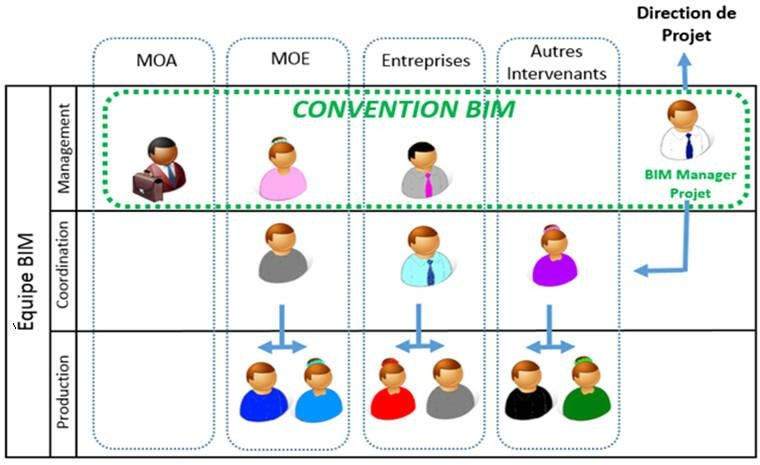
\includegraphics[width=0.84\textwidth]{pics/convention_bim_acteurs.png}
    \caption{Acteurs et organisation d'une démarche BIM collaborative}
\end{figure}

% ------------------------------------------------------------
\section{Missions confiées durant le PFE}

Les missions confiées durant le PFE s'articulent autour de plusieurs axes complémentaires. Elles ne se limitent pas au développement informatique, mais couvrent également la modélisation BIM, l'analyse métier, l'automatisation et l'intégration numérique.

\begin{table}[H]
\centering
\caption{Missions principales confiées durant le PFE}
\begin{tabularx}{0.95\textwidth}{|L{4.2cm}|Y|}
\hline
\textbf{Mission} & \textbf{Description} \\
\hline
Contribution à la modélisation BIM C2R & Participation à l'organisation et à la modélisation des maquettes architecture, structure, fluides, CFO, CFA et synthèse. \\
\hline
Analyse du besoin métier & Étude du processus de traitement des réservations structurelles et identification des limites du workflow existant. \\
\hline
Développement de RESBIM & Conception et développement d'un plugin Revit pour automatiser la génération, le suivi et la vérification des réservations. \\
\hline
Intégration BIM--IoT & Mise en œuvre d'une chaîne ESP32, MQTT, Node-RED et Revit pour la supervision technique d'équipements. \\
\hline
Valorisation innovation & Participation au challenge d'innovation VEAO VINCI avec le projet RESBIM. \\
\hline
\end{tabularx}
\end{table}

% ------------------------------------------------------------
\section{Planification générale du PFE}

La réalisation du PFE a été organisée selon une progression logique : compréhension du contexte, analyse du besoin, modélisation BIM, prototypage, développement, intégration BIM--IoT, validation, analyse des résultats et rédaction du rapport.

\begin{table}[H]
\centering
\caption{Planification synthétique du projet de fin d'études}
\begin{tabularx}{0.95\textwidth}{|L{3.5cm}|L{3.2cm}|Y|}
\hline
\textbf{Phase} & \textbf{Période indicative} & \textbf{Travaux réalisés} \\
\hline
Cadrage et compréhension du besoin & Janvier 2026 & Analyse du contexte BIM, compréhension du processus de synthèse et identification du besoin lié aux réservations. \\
\hline
Modélisation BIM du projet C2R & Janvier--février 2026 & Contribution aux maquettes architecture, structure, fluides, CFO, CFA et synthèse. \\
\hline
Prototypage et règles métier & Février 2026 & Premiers essais avec Dynamo pour tester les logiques de détection, fusion, alertes et nomenclatures. \\
\hline
Développement RESBIM & Février--avril 2026 & Développement du plugin Revit en C\# : ruban, commandes, génération, vérification, statuts, nomenclature et XML. \\
\hline
Intégration BIM--IoT & Avril--mai 2026 & Mise en œuvre de l'architecture ESP32, MQTT, Node-RED et Revit pour la supervision technique. \\
\hline
Validation et résultats & Mai 2026 & Tests fonctionnels, exploitation du fichier Excel, comparaison avant/après et analyse de la valeur ajoutée. \\
\hline
Rédaction et préparation soutenance & Mai--juin 2026 & Structuration du rapport, préparation des captures, annexes, résultats et support de soutenance. \\
\hline
\end{tabularx}
\end{table}

% ------------------------------------------------------------
\section{Conclusion}

Ce chapitre a permis de présenter l'environnement industriel du projet, depuis le groupe VINCI jusqu'à la cellule BIM \& Synthèse de VINCI Energies Building Solutions. La diversité des lots techniques, l'exigence de coordination entre disciplines et la nécessité de fiabiliser les livrables BIM justifient pleinement le développement d'une solution dédiée à l'automatisation des réservations structurelles.

Le chapitre suivant présente la problématique générale et l'analyse du besoin, en mettant en évidence les limites du processus actuel et les objectifs fonctionnels attendus de RESBIM.
% ============================================================
% CHAPITRE 2
% ============================================================
\chapter{Problématique générale et analyse du besoin}

\section{Introduction}
Ce chapitre formalise le besoin métier avant le développement de la solution. Il présente le contexte des réservations structurelles, le processus actuel, les limites observées, les besoins fonctionnels et la problématique finale du PFE. L'état de l'art est volontairement placé après ce chapitre afin de partir d'abord du problème réel rencontré dans l'entreprise.

\section{Contexte métier des réservations structurelles}
Dans les projets BIM multidisciplinaires, les réseaux techniques MEP traversent fréquemment les éléments structurels tels que les voiles et les dalles. Ces traversées doivent être anticipées afin d'éviter les conflits en phase d'exécution. La réservation structurelle représente donc l'ouverture nécessaire pour permettre le passage d'une canalisation, d'une gaine, d'un chemin de câbles ou d'un ensemble technique.

Une réservation n'est pas uniquement un objet géométrique. Elle doit contenir des informations exploitables : forme, dimensions, niveau, support, lot, numéro, statut, commentaire, origine du réseau et état de validation. Elle constitue ainsi un objet de synthèse entre plusieurs intervenants : BIM coordinateur, modèleur MEP, structure, chantier et responsables de validation.

\insertfigure[0.82\textwidth]{pics/fig_reservation_principe.png}{Principe d'une réservation structurelle dans la coordination MEP--Structure}
\insertfigure[0.82\textwidth]{pics/fig_conflit_vers_reservation.png.jpg}{Transformation d'un conflit MEP--Structure en objet de réservation}

\section{Processus actuel de traitement des réservations}
Le processus classique repose sur une chaîne de travail composée de plusieurs étapes :
\begin{enumerate}[leftmargin=1.2cm]
    \item modélisation des réseaux techniques dans les maquettes MEP ;
    \item liaison avec la maquette structure ;
    \item détection des conflits entre réseaux et supports structurels ;
    \item analyse des conflits par le coordinateur BIM ;
    \item création ou modification des réservations dans Revit ;
    \item vérification des dimensions, du niveau, du support et de l'orientation ;
    \item suivi par vues, commentaires, nomenclatures ou échanges entre intervenants.
\end{enumerate}

\begin{figure}[H]
\centering
\begin{tikzpicture}[
    node distance=0.8cm and 0.8cm,
    process/.style={
        draw=vinciBlue,
        rounded corners=4pt,
        thick,
        align=center,
        fill=lightGray,
        text width=0.24\textwidth,
        minimum height=1.35cm,
        font=\small
    },
    arrow/.style={
        -{Latex[length=2.8mm,width=2mm]},
        thick,
        draw=vinciBlue
    }
]
\node[process] (a) {1. MODELISATION\\MEP};
\node[process, right=of a] (b) {2. LIAISON\\STRUCTURE};
\node[process, right=of b] (c) {3. DETECTION DES\\CONFLITS};
\node[process, below=of c] (d) {4. ANALYSE\\BIM};
\node[process, left=of d] (e) {5. CREATION DES\\RESERVATIONS};
\node[process, left=of e] (f) {6. VERIFICATION\\ET CONTROLE};
\node[process, below=of b] (g) {7. SUIVI ET\\COORDINATION};

\draw[arrow] (a) -- (b);
\draw[arrow] (b) -- (c);
\draw[arrow] (c) -- (d);
\draw[arrow] (d) -- (e);
\draw[arrow] (e) -- (f);
\draw[arrow] (f.east) -- ++(0.35,0) |- (g.west);
\end{tikzpicture}
\caption{Processus actuel de traitement des réservations structurelles}
\end{figure}

\section{Limites du processus existant}
Le processus existant présente plusieurs limites :
\begin{itemize}[leftmargin=1.2cm]
    \item temps élevé de traitement lorsque le nombre de traversées est important ;
    \item dépendance à l'expérience de l'utilisateur ;
    \item risque d'oubli de certaines réservations ;
    \item erreurs possibles de dimensions, de niveau, de support ou d'orientation ;
    \item difficulté à assurer une traçabilité complète ;
    \item absence de standardisation forte entre utilisateurs ou projets ;
    \item difficulté à préserver les réservations déjà validées ;
    \item suivi visuel et documentaire parfois dispersé.
\end{itemize}

\section{Analyse du besoin}
L'analyse du besoin montre que la solution attendue doit couvrir l'ensemble du workflow des réservations, et non uniquement la détection des conflits. Elle doit permettre de générer automatiquement les réservations, de gérer les cas particuliers, de structurer les informations et de faciliter la vérification.

\begin{table}[H]
\centering
\caption{Analyse du besoin fonctionnel lié aux réservations}
\begin{tabularx}{0.95\textwidth}{|L{4.6cm}|Y|}
\hline
\textbf{Besoin identifié} & \textbf{Fonction attendue dans la solution} \\
\hline
Réduire le traitement manuel & Génération automatique des réservations depuis les intersections MEP--Structure. \\
\hline
Travailler par périmètre contrôlé & Génération par niveau ou dans un espace cible. \\
\hline
Gérer les cas particuliers & Génération manuelle assistée avec familles et paramètres standardisés. \\
\hline
Éviter les doublons & Fusion des réservations compatibles ou proches. \\
\hline
Contrôler les résultats & Vérification guidée réservation par réservation. \\
\hline
Suivre les états & Paramètres de statut et filtres de couleurs. \\
\hline
Identifier les objets & Numérotation automatique et étiquetage. \\
\hline
Exploiter les informations & Nomenclatures et échange XML. \\
\hline
Préserver les décisions validées & Verrouillage et conservation des réservations validées. \\
\hline
\end{tabularx}
\end{table}

\section{Cahier des charges fonctionnel}
Le cahier des charges fonctionnel de RESBIM est défini autour des fonctions suivantes :
\begin{itemize}[leftmargin=1.2cm]
    \item génération automatique des réservations ;
    \item génération par niveau ;
    \item génération dans un espace ou une zone ;
    \item génération manuelle assistée ;
    \item gestion des cas voile et dalle ;
    \item gestion des formes circulaires et rectangulaires ;
    \item calcul des dimensions et majorations ;
    \item placement et orientation ;
    \item fusion des réservations ;
    \item vérification guidée ;
    \item validation, verrouillage et suppression contrôlée ;
    \item numérotation et étiquetage ;
    \item filtres de couleurs ;
    \item nomenclature ;
    \item export et import XML.
\end{itemize}

\section{Extension du besoin vers la supervision technique}
Au-delà du traitement des réservations, le PFE explore une extension de la maquette BIM vers la supervision technique. Cette extension constitue un second axe complémentaire au travail RESBIM. Elle cherche à montrer qu'une maquette bien structurée ne doit pas rester un simple support de conception et de coordination, mais qu'elle peut aussi évoluer vers un support de visualisation, de suivi et d'aide à la décision.

\subsection{Limites d'une maquette BIM statique}
Une maquette BIM, même correctement modélisée et coordonnée, reste limitée si elle est utilisée uniquement comme support graphique ou documentaire. Dans les bâtiments techniques, les besoins d'exploitation dépassent la simple représentation géométrique. Les responsables techniques ont également besoin de suivre l'état réel des équipements, de repérer rapidement une anomalie et de relier une alerte à son emplacement dans le bâtiment.

\subsection{Intérêt d'une intégration BIM--IoT}
L'intégration BIM--IoT permet de relier des objets BIM à des données issues du terrain ou d'une chaîne de supervision. Ce couplage ouvre la voie à une lecture dynamique de la maquette, dans laquelle les équipements peuvent être associés à des mesures, des statuts, des événements et des alarmes. Dans cette logique, Revit ne sert plus seulement à modéliser, mais aussi à contextualiser l'information technique dans un environnement spatial cohérent.

\subsection{Besoin de supervision pour les bâtiments techniques}
Les bâtiments techniques, comme les Data Centers, contiennent des équipements sensibles : baies serveurs, tableaux électriques, équipements CVC, sprinklers et équipements de sécurité. Le suivi de variables comme la température, l'humidité, l'alimentation électrique ou les états d'alarme devient alors essentiel. La possibilité de connecter ces objets BIM à des données issues d'un ESP32, transmises via MQTT et orchestrées par Node-RED, permet d'utiliser la maquette comme support de supervision technique et de visualisation des états en temps quasi réel.

\section{Problématique finale}
La problématique du PFE peut être formulée comme suit :

\importantbox{
\textbf{Comment concevoir et développer une solution BIM intégrée permettant, d'une part, d'automatiser la génération, le dimensionnement, la vérification et le suivi des réservations structurelles afin de réduire le temps de traitement et d'améliorer la traçabilité dans une maquette Revit multidisciplinaire, et, d'autre part, d'étendre cette maquette vers une logique BIM--IoT capable de relier les objets techniques à des données terrain pour la supervision dynamique des bâtiments ?}
}

\section{Objectifs spécifiques}
\subsection{Objectifs spécifiques liés à RESBIM}
Les objectifs spécifiques du premier axe sont les suivants :
\begin{itemize}[leftmargin=1.2cm]
    \item analyser le processus existant de traitement des réservations ;
    \item participer à la modélisation et à la préparation de la maquette C2R ;
    \item développer un plugin Revit structuré et utilisable par la cellule BIM \& Synthèse ;
    \item intégrer les règles métier de dimensionnement, placement, fusion, vérification et suivi ;
    \item améliorer la traçabilité, la visualisation et l'exploitation des réservations dans la maquette ;
    \item mesurer les gains à travers des indicateurs issus d'un fichier Excel.
\end{itemize}

\subsection{Objectifs spécifiques liés à l'intégration BIM--IoT}
Les objectifs spécifiques du second axe sont les suivants :
\begin{itemize}[leftmargin=1.2cm]
    \item définir une chaîne BIM--IoT basée sur ESP32, MQTT, Node-RED et Revit ;
    \item relier les objets techniques de la maquette à des données issues du terrain ou simulées ;
    \item permettre la visualisation des états, événements et alertes dans un contexte spatial BIM cohérent ;
    \item explorer l'usage de la maquette comme support de supervision dynamique pour les bâtiments techniques ;
    \item valoriser le projet dans une logique d'innovation interne.
\end{itemize}

\section{Conclusion}
L'analyse du besoin montre que le véritable enjeu n'est pas seulement de détecter les conflits, mais de transformer un processus manuel et dispersé en workflow Revit intégré, contrôlable et traçable. Le chapitre suivant présente les concepts techniques nécessaires pour situer la solution dans son cadre scientifique et technologique.

% ============================================================
% CHAPITRE 3
% ============================================================
\chapter{État de l'art et concepts techniques utilisés}

\section{Introduction}
Ce chapitre présente les notions nécessaires pour comprendre les trois axes du PFE : le BIM, la coordination MEP--Structure, l'automatisation sous Revit et l'intégration BIM--IoT. L'objectif n'est pas de produire un état de l'art trop général, mais de retenir uniquement les concepts directement utiles au projet.

\section{Building Information Modeling}
Le Building Information Modeling est une méthode de travail fondée sur une maquette numérique informée. Contrairement à une représentation 3D simple, une maquette BIM contient des objets paramétriques associés à des données : dimensions, niveaux, matériaux, systèmes, identifiants, statuts, classifications et informations de suivi.

Dans un projet technique, le BIM permet de centraliser l'information, de coordonner les disciplines et de réduire les incohérences entre livrables. Il devient un support de conception, de synthèse, de contrôle et progressivement d'exploitation.

\insertfigure[0.78\textwidth]{pics/cycle_vie_bim.png}{Cycle de vie BIM}
\insertfigure[0.78\textwidth]{pics/dimensions_bim.png}{Dimensions du BIM}

\section{Coordination BIM multidisciplinaire}
La coordination BIM multidisciplinaire consiste à organiser la cohabitation entre les maquettes architecture, structure, fluides, CFO, CFA et autres disciplines. Elle permet de vérifier la cohérence géométrique et informationnelle entre les lots avant la phase chantier.

Cette coordination est particulièrement importante pour les lots techniques, car les réseaux MEP occupent des volumes importants et traversent fréquemment les éléments structurels. La maquette de synthèse devient alors le lieu principal de contrôle et de décision.

\insertfigure[0.82\textwidth]{pics/coordination_multidisciplinaire.png}{Organisation d'une coordination BIM multidisciplinaire}

\section{Coordination MEP--Structure et réservations}
La coordination MEP--Structure porte sur les interactions entre les réseaux techniques et les supports structurels. Lorsqu'une canalisation, une gaine ou un chemin de câbles traverse un voile ou une dalle, une réservation doit être prévue.

Les réservations peuvent être :
\begin{itemize}[leftmargin=1.2cm]
    \item circulaires, principalement pour les canalisations ;
    \item rectangulaires, principalement pour les gaines, chemins de câbles ou ensembles techniques ;
    \item associées à un voile ou à une dalle selon le support traversé.
\end{itemize}

\insertfigure[0.82\textwidth]{pics/principe_reservation_voile.png}{Principe d'une réservation dans un voile}
\insertfigure[0.82\textwidth]{pics/principe_reservation_dalle.png}{Principe d'une réservation dans une dalle}

\section{Clash detection et synthèse technique}
La \textit{clash detection} permet d'identifier les conflits géométriques entre éléments de différentes disciplines. Des outils comme Navisworks ou Revit permettent de repérer les collisions entre réseaux techniques et éléments structurels. Cependant, la détection du conflit ne suffit pas : il faut ensuite transformer cette information en réservation exploitable, correctement dimensionnée et suivie.



\section{Automatisation BIM sous Revit}
L'automatisation BIM consiste à déléguer à un script ou à un plugin les tâches répétitives et normalisables. Dans le cadre de ce PFE, elle concerne principalement le traitement des réservations structurelles.

Dynamo permet de prototyper rapidement des logiques de traitement visuel. L'API Revit permet d'accéder aux éléments, familles, paramètres, vues et transactions. Le développement en C\# permet de construire un plugin intégré à l'interface Revit, plus robuste, plus maintenable et mieux adapté à une utilisation métier.

\insertfigure[0.82\textwidth]{pics/automatisation_revit.png}{Principe d'automatisation sous Revit}
\insertfigure[0.82\textwidth]{pics/dev_revit_dynamo_exemple.png}{Dynamo et API Revit dans une démarche d'automatisation}

\section{BIM--IoT et supervision technique}
L'intégration BIM--IoT consiste à relier des objets BIM à des données issues de capteurs ou d'équipements connectés. Cette approche permet de visualiser des mesures, états ou alarmes directement dans le contexte spatial de la maquette.

Dans ce PFE, l'intégration repose sur :
\begin{itemize}[leftmargin=1.2cm]
    \item l'ESP32 pour l'acquisition ou la communication des données ;
    \item MQTT comme protocole léger de transport des messages ;
    \item Node-RED pour l'injection, le traitement ou le routage des flux ;
    \item Revit et le plugin C\# pour la mise à jour des paramètres et la visualisation.
\end{itemize}

\insertfigure[0.82\textwidth]{pics/architecture_generale_bim_iot.png}{Architecture générale BIM--IoT}

\section{Synthèse de l'état de l'art}
\begin{table}[H]
\centering
\caption{Synthèse des concepts techniques mobilisés}
\begin{tabularx}{0.95\textwidth}{|L{4.0cm}|Y|}
\hline
\textbf{Domaine} & \textbf{Apport pour le PFE} \\
\hline
BIM & Support de modélisation, coordination et structuration de la donnée. \\
\hline
Coordination MEP--Structure & Base du problème des réservations dans les voiles et dalles. \\
\hline
Clash detection & Identification des conflits entre réseaux et structure. \\
\hline
Dynamo & Prototypage rapide des règles métier avant développement. \\
\hline
API Revit / C\# & Développement d'un plugin intégré, maintenable et industrialisable. \\
\hline
BIM--IoT & Extension de la maquette vers la supervision technique. \\
\hline
\end{tabularx}
\end{table}

\section{Conclusion}
L'état de l'art montre que les outils BIM et les technologies d'automatisation existent, mais qu'un besoin persiste : relier la détection, la génération, le suivi et la vérification des réservations dans un workflow complet. Cette conclusion justifie le développement de RESBIM et l'ouverture vers une maquette connectée par l'intégration BIM--IoT.

% ============================================================
% CHAPITRE 4
% ============================================================
\chapter{Contribution à la modélisation BIM du projet C2R}

\section{Introduction}
Ce chapitre présente la contribution réalisée sur la modélisation BIM du projet C2R. Cette partie est indépendante du développement RESBIM et de l'intégration BIM--IoT. Elle correspond à un travail de production et d'organisation des maquettes qui a permis de mieux comprendre les contraintes réelles de coordination.

\section{Présentation du projet C2R}
Le projet C2R constitue le cas support principal de la contribution BIM. Il regroupe plusieurs disciplines : architecture, structure, fluides, CFO, CFA et synthèse. Cette organisation permet d'observer les interactions entre les lots et d'identifier les zones où la coordination est nécessaire.

\insertfigure[0.92\textwidth]{pics/vue_3d_c2r.png}{Vue 3D générale du projet C2R}

\section{Organisation des maquettes par discipline}
Le projet est organisé autour de maquettes disciplinaires liées dans un environnement de synthèse. Cette séparation permet de préserver les responsabilités par lot tout en permettant une coordination globale.

\begin{table}[H]
\centering
\caption{Organisation des maquettes du projet C2R}
\begin{tabularx}{0.95\textwidth}{|L{3.8cm}|Y|}
\hline
\textbf{Maquette} & \textbf{Rôle dans la coordination} \\
\hline
Architecture & Référence spatiale : locaux, murs, portes, fenêtres, sols et organisation des niveaux. \\
\hline
Structure & Support porteur : voiles, dalles, poutres, poteaux et éléments concernés par les réservations. \\
\hline
Fluides & Réseaux techniques : canalisations, gaines, CVC, plomberie et passages techniques. \\
\hline
CFO & Réseaux courant fort : chemins de câbles, tableaux, passages électriques et équipements associés. \\
\hline
CFA & Réseaux courant faible : communication, sécurité, détection, chemins de câbles et équipements faibles. \\
\hline
Synthèse & Regroupement des liens pour la coordination multidisciplinaire et la détection des conflits. \\
\hline
\end{tabularx}
\end{table}

\insertfigure[0.92\textwidth]{pics/organisation_liens_revit_c2r.png}{Organisation des liens Revit du projet C2R}

\section{Modélisation architecture}
La modélisation architecture comprend les éléments servant de référence spatiale : murs, portes, fenêtres, sols, niveaux et locaux. Cette maquette permet de comprendre la configuration générale du bâtiment, la répartition des espaces et les zones techniques.

\insertfigure[0.86\textwidth]{pics/maquette_architecture_c2r.png}{Maquette architecture du projet C2R}
\insertfigure[0.86\textwidth]{pics/niveau_architecture_c2r.png}{Exemple de niveau architectural du projet C2R}

\section{Modélisation structure}
La modélisation structure concerne les éléments porteurs : voiles, dalles, poteaux, poutres et niveaux structurels. Cette discipline est centrale pour le sujet RESBIM, car les réservations sont générées dans les voiles et les dalles lorsque les réseaux MEP les traversent.

\insertfigure[0.86\textwidth]{pics/maquette_structure_c2r.png}{Maquette structure du projet C2R}
\insertfigure[0.86\textwidth]{pics/voiles_dalles_c2r.png}{Voiles et dalles concernés par la coordination MEP--Structure}

\section{Modélisation fluides}
La modélisation fluides comprend les canalisations, gaines, réseaux CVC, plomberie et passages techniques. Ces réseaux peuvent générer des réservations circulaires lorsqu'il s'agit de canalisations ou rectangulaires lorsqu'il s'agit de gaines.

\insertfigure[0.86\textwidth]{pics/reseaux_fluides_c2r.png}{Réseaux fluides du projet C2R}
\insertfigure[0.86\textwidth]{pics/passage_canalisation_voile.png}{Exemple de canalisation traversant un voile}
\insertfigure[0.86\textwidth]{pics/passage_gaine_dalle.png}{Exemple de gaine traversant une dalle}

\section{Modélisation CFO}
La modélisation CFO est intégrée dans ce chapitre, car elle fait partie de la contribution BIM C2R. Elle concerne les réseaux de courant fort : chemins de câbles, tableaux électriques, équipements électriques et passages associés. Les chemins de câbles CFO peuvent générer des besoins de réservations rectangulaires lorsqu'ils traversent des voiles ou dalles.

\insertfigure[0.86\textwidth]{pics/reseaux_cfo_c2r.png}{Réseaux CFO du projet C2R}
\insertfigure[0.86\textwidth]{pics/chemins_cables_cfo_c2r.png}{Chemins de câbles CFO et coordination avec la structure}

\section{Modélisation CFA}
La modélisation CFA est également placée dans ce chapitre, séparée de RESBIM et du BIM--IoT. Elle concerne les réseaux de courant faible : communication, sécurité, détection, vidéosurveillance, câblage faible et chemins de câbles CFA. Ces éléments doivent être intégrés à la maquette de synthèse afin de vérifier leurs interfaces avec la structure et les autres lots.

\insertfigure[0.86\textwidth]{pics/reseaux_cfa_c2r.png}{Réseaux CFA du projet C2R}
\insertfigure[0.86\textwidth]{pics/chemins_cables_cfa_c2r.png}{Chemins de câbles CFA dans la maquette}

\section{Maquette de synthèse}
La maquette de synthèse regroupe les disciplines afin de contrôler les interfaces entre les lots. Elle permet de visualiser simultanément l'architecture, la structure, les fluides, le CFO et le CFA. Elle constitue l'environnement de coordination principal.

\insertfigure[0.92\textwidth]{pics/maquette_synthese_c2r.png}{Maquette de synthèse du projet C2R}
\insertfigure[0.92\textwidth]{pics/vue_multidisciplinaire_c2r.png}{Vue multidisciplinaire ARC/STR/FLU/CFO/CFA}

\section{Préparation des vues et gabarits de contrôle}
La préparation des vues et gabarits facilite la lecture de la maquette et la vérification des interfaces. Les vues peuvent être organisées par niveau, par discipline, par zone ou par objectif de contrôle.

Les gabarits de vue permettent d'uniformiser l'affichage, de filtrer les catégories, de mettre en évidence les réseaux techniques et d'isoler les zones nécessitant une vérification.

\insertfigure[0.86\textwidth]{pics/gabarit_vue_coordination_c2r.png}{Gabarit de vue de coordination}
\insertfigure[0.86\textwidth]{pics/vue_controle_multidisciplinaire_c2r.png}{Vue de contrôle multidisciplinaire}

\section{Livrables BIM produits}
\begin{table}[H]
\centering
\caption{Livrables BIM produits dans le cadre du projet C2R}
\begin{tabularx}{0.95\textwidth}{|L{4.0cm}|L{4.0cm}|Y|}
\hline
\textbf{Livrable} & \textbf{Rôle} & \textbf{Utilisation} \\
\hline
Maquette architecture & Référence spatiale & Coordination des locaux et niveaux. \\
\hline
Maquette structure & Supports porteurs & Analyse des voiles, dalles et traversées. \\
\hline
Maquette fluides & Réseaux techniques & Identification des passages MEP. \\
\hline
Maquette CFO & Courant fort & Coordination des chemins de câbles et équipements électriques. \\
\hline
Maquette CFA & Courant faible & Coordination des réseaux faibles et chemins de câbles CFA. \\
\hline
Maquette synthèse & Regroupement multi-lots & Contrôle global des interfaces. \\
\hline
Vues et gabarits & Standardisation visuelle & Vérification rapide par niveau, discipline ou zone. \\
\hline
\end{tabularx}
\end{table}

\section{Conclusion}
La contribution à la modélisation C2R constitue une partie séparée et importante du PFE. Elle a permis de produire, organiser et contrôler les maquettes architecture, structure, fluides, CFO, CFA et synthèse. Ce travail a aussi fourni un contexte réaliste pour comprendre les besoins de coordination, sans être confondu avec le développement RESBIM ou l'intégration BIM--IoT.

% ============================================================
% CHAPITRE 5
% ============================================================
\chapter{Conception et développement de RESBIM}

\section{Introduction}
Ce chapitre présente la contribution principale du PFE : la conception et le développement du plugin RESBIM. Il regroupe la phase de prototypage Dynamo, la préparation des familles et paramètres, l'architecture fonctionnelle et technique, ainsi que les modules développés sous Revit en C\#.

\section{Passage du besoin métier vers une solution Revit}
L'analyse du besoin a montré que le traitement manuel des réservations doit être remplacé par un workflow intégré dans Revit. Le choix d'un plugin permet de réduire les allers-retours entre outils, de limiter les manipulations répétitives, de structurer les données, d'améliorer la traçabilité et de fournir une interface accessible à la cellule BIM \& Synthèse.

\section{Phase de prototypage avec Dynamo}
Avant le développement C\#, Dynamo a été utilisé pour prototyper rapidement certaines règles métier. Cette phase a permis de tester des logiques de détection, d'alerte, de fusion, de génération et de préparation de nomenclatures.

\begin{table}[H]
\centering
\caption{Scripts Dynamo réalisés dans la phase de prototypage}
\begin{tabularx}{0.95\textwidth}{|L{4.4cm}|Y|}
\hline
\textbf{Script} & \textbf{Rôle principal} \\
\hline
\texttt{Alerte\_RES.dyn} & Identification de cas nécessitant une vérification. \\
\hline
\texttt{Alerte\_RES\_EGM.dyn} & Gestion d'alertes spécifiques liées aux réservations. \\
\hline
\texttt{FusionAuto.dyn} & Fusion automatique de réservations compatibles. \\
\hline
\texttt{FusionManuel.dyn} & Fusion assistée par l'utilisateur pour les cas particuliers. \\
\hline
\texttt{RES\_ScheduleView.dyn} & Préparation de vues et nomenclatures de contrôle. \\
\hline
\texttt{RES\_script1.0.dyn} & Premiers essais de génération et traitement des réservations. \\
\hline
Scripts de raccords et itérations intermédiaires & Ajustement de règles métier avant migration vers C\#. \\
\hline
\end{tabularx}
\end{table}

\insertfigure[0.86\textwidth]{pics/script_dynamo_alerte_res.png}{Script Dynamo de détection ou alerte}
\insertfigure[0.86\textwidth]{pics/script_dynamo_fusion.png}{Script Dynamo de fusion}
\insertfigure[0.86\textwidth]{pics/script_dynamo_schedule.png}{Script Dynamo de préparation des nomenclatures}
\insertfigure[0.86\textwidth]{pics/resultat_dynamo_revit.png}{Résultat obtenu dans Revit après exécution Dynamo}

\section{Limites du prototypage Dynamo}
Dynamo a été utile pour tester les règles métier, mais il présente des limites pour un usage industriel :
\begin{itemize}[leftmargin=1.2cm]
    \item scripts longs et difficiles à maintenir ;
    \item interface peu adaptée à un utilisateur final ;
    \item gestion des erreurs moins robuste ;
    \item dépendance à la structure de la maquette ;
    \item difficulté à organiser plusieurs fonctionnalités dans un workflow unique ;
    \item absence d'un ruban Revit professionnel ;
    \item difficulté à intégrer connexion, vérification guidée, XML, statuts et numérotation.
\end{itemize}

Ces limites justifient le passage vers un plugin C\# structuré.

\section{Vision générale de RESBIM}
RESBIM est conçu comme un outil métier intégré à Revit. Il couvre la chaîne complète :
\begin{center}
\textbf{Détection} $\rightarrow$ \textbf{choix de famille} $\rightarrow$ \textbf{dimensionnement} $\rightarrow$ \textbf{placement} $\rightarrow$ \textbf{orientation} $\rightarrow$ \textbf{paramètres} $\rightarrow$ \textbf{fusion} $\rightarrow$ \textbf{vérification} $\rightarrow$ \textbf{couleurs} $\rightarrow$ \textbf{nomenclature} $\rightarrow$ \textbf{XML}
\end{center}

\insertfigure[0.92\textwidth]{pics/vision_globale_resbim.png}{Vision globale de RESBIM}

\section{Architecture fonctionnelle}
L'architecture fonctionnelle du plugin repose sur plusieurs modules :
\begin{itemize}[leftmargin=1.2cm]
    \item connexion et accès utilisateur ;
    \item génération automatique ;
    \item génération par niveau ;
    \item génération dans un espace ;
    \item génération manuelle assistée ;
    \item fusion des réservations ;
    \item vérification guidée ;
    \item visualisation par couleurs ;
    \item numérotation et étiquetage ;
    \item nomenclature ;
    \item export et import XML.
\end{itemize}

\insertfigure[0.92\textwidth]{pics/architecture_fonctionnelle_resbim.png}{Architecture fonctionnelle du plugin RESBIM}

\section{Architecture technique C\# / Revit API}
Le projet C\# est organisé par responsabilités afin de faciliter la maintenance et l'évolution du code :
\begin{itemize}[leftmargin=1.2cm]
    \item \texttt{Commands} : points d'entrée des boutons du ruban ;
    \item \texttt{Workflows} : orchestration des traitements ;
    \item \texttt{Models} : structures de données ;
    \item \texttt{Services} : détection, dimensionnement, placement, paramètres, fusion, XML ;
    \item \texttt{UI} : fenêtres, panneaux et composants d'interface ;
    \item \texttt{Utils} : conversions d'unités, méthodes auxiliaires ;
    \item \texttt{Constants} : noms de paramètres, familles, statuts et valeurs constantes.
\end{itemize}

\insertfigure[0.92\textwidth]{pics/architecture_technique_csharp_resbim.png}{Architecture technique du projet C\# RESBIM}

\section{Développement du ruban RESBIM}
Le plugin se présente sous la forme d'un onglet \texttt{RESBIM} dans le ruban Revit. Les commandes sont regroupées selon leur rôle : accès, création, contrôle, visualisation et données.

\insertfigure[0.92\textwidth]{pics/fig_resbim_ruban_complet.png}{Ruban complet RESBIM}
\insertfigure[0.92\textwidth]{pics/groupes_commandes_resbim.png}{Groupes de commandes RESBIM}

\section{Familles et paramètres intégrés dans RESBIM}
Les familles et paramètres sont inclus dans le chapitre RESBIM, car ils font partie de l'implémentation de l'outil. Le plugin s'appuie sur des familles adaptées aux cas de voiles et de dalles.

\begin{longtable}{|L{5.2cm}|L{8.2cm}|}
\caption{Familles de réservations utilisées par RESBIM}\\
\hline
\textbf{Famille} & \textbf{Rôle} \\
\hline
\texttt{CEG\_RES\_CIRC\_VOILE} & Réservation circulaire destinée aux voiles. \\
\hline
\texttt{CEG\_RES\_RECT\_VOILE} & Réservation rectangulaire destinée aux voiles. \\
\hline
\texttt{CEG\_RES\_CIRC\_DALLE} & Réservation circulaire destinée aux dalles. \\
\hline
\texttt{CEG\_RES\_RECT\_DALLE} & Réservation rectangulaire destinée aux dalles. \\
\hline
\texttt{CEG\_ETIQ\_RES} & Étiquette de réservation pour afficher numéro, dimensions et statut. \\
\hline
\end{longtable}

\begin{table}[H]
\centering
\caption{Paramètres exploités par RESBIM}
\begin{tabularx}{0.95\textwidth}{|L{4.0cm}|Y|}
\hline
\textbf{Famille de paramètres} & \textbf{Exemples et rôle} \\
\hline
Identification & \texttt{CEG\_ID}, \texttt{CEG\_NUMERO}, \texttt{CEG\_TYPE}, \texttt{CEG\_LOT}. \\
\hline
Traçabilité & \texttt{CEG\_ID\_MEP\_PRINCIPAL}, \texttt{CEG\_ID\_SUPPORT}, \texttt{CEG\_DATE\_CREATION}, \texttt{CEG\_CREE\_PAR}. \\
\hline
Statuts & \texttt{CEG\_VALIDE}, \texttt{CEG\_A\_VERIFIER}, \texttt{CEG\_VERROUILLER}, \texttt{CEG\_ON\_HOLD}, \texttt{CEG\_STATUT}. \\
\hline
Géométrie & Longueur, hauteur, épaisseur, diamètre et élévation. \\
\hline
Commentaires & \texttt{CEG\_COMMENTAIRE}, commentaire de fusion et remarques de vérification. \\
\hline
\end{tabularx}
\end{table}

\insertfigure[0.86\textwidth]{pics/familles_resbim.png}{Familles de réservations RESBIM}
\insertfigure[0.86\textwidth]{pics/parametres_partages_resbim.png}{Paramètres partagés utilisés par RESBIM}

\section{Module de génération automatique}
Le module de génération automatique représente le cœur de RESBIM. Son workflow est le suivant :
\begin{enumerate}[leftmargin=1.2cm]
    \item choix du niveau ou de la zone ;
    \item récupération des éléments MEP ;
    \item récupération des supports structurels ;
    \item détection des intersections ;
    \item classification du passage : circulaire ou rectangulaire ;
    \item choix du support : voile ou dalle ;
    \item choix de la famille ;
    \item calcul des dimensions avec majoration ;
    \item placement et orientation ;
    \item écriture des paramètres ;
    \item application du statut initial.
\end{enumerate}

\insertfigure[0.92\textwidth]{pics/workflow_generation_automatique_resbim.png}{Workflow de génération automatique des réservations}

\section{Génération des réservations en voiles}
Lorsqu'un réseau traverse un voile, RESBIM identifie le point d'intersection, calcule les dimensions nécessaires, choisit la famille correspondante et place la réservation dans le support. Une canalisation conduit généralement à une réservation circulaire, tandis qu'une gaine ou un chemin de câbles conduit à une réservation rectangulaire.

\insertfigure[0.86\textwidth]{pics/canalisation_traversant_voile.png}{Canalisation traversant un voile avant génération}
\insertfigure[0.86\textwidth]{pics/reservation_circulaire_voile_generee.png}{Réservation circulaire générée dans un voile}
\insertfigure[0.86\textwidth]{pics/gaine_traversant_voile.png}{Gaine traversant un voile avant génération}
\insertfigure[0.86\textwidth]{pics/reservation_rectangulaire_voile_generee.png}{Réservation rectangulaire générée dans un voile}

\section{Génération des réservations en dalles}
Pour les dalles, RESBIM traite les réseaux qui traversent verticalement ou avec une inclinaison nécessitant une ouverture. Le plugin choisit une famille de dalle, récupère l'épaisseur du support, place l'instance au bon niveau et écrit les dimensions calculées.

\insertfigure[0.86\textwidth]{pics/reseau_traversant_dalle.png}{Réseau traversant une dalle}
\insertfigure[0.86\textwidth]{pics/reservation_dalle_generee.png}{Réservation générée dans une dalle}

\section{Module de génération manuelle assistée}
Certains cas particuliers nécessitent une intervention de l'utilisateur. La génération manuelle assistée permet de créer une réservation en conservant la standardisation imposée par RESBIM : choix de la famille, dimensions, statut, commentaire, numéro et paramètres de traçabilité.

\insertfigure[0.86\textwidth]{pics/fenetre_generation_manuelle_resbim.png}{Fenêtre de génération manuelle assistée}

\section{Module de fusion des réservations}
Le module de fusion permet de réduire les doublons et d'améliorer la lisibilité de la maquette. Il regroupe les réservations compatibles ou superposées selon les règles définies, puis conserve les informations nécessaires dans les paramètres et commentaires.

\insertfigure[0.86\textwidth]{pics/reservations_avant_fusion.png}{Réservations avant fusion}
\insertfigure[0.86\textwidth]{pics/reservation_apres_fusion.png}{Réservation après fusion}

\section{Module de vérification guidée}
La vérification guidée constitue un module central pour fiabiliser le workflow. Elle permet de parcourir les réservations, consulter leurs paramètres, modifier les commentaires, valider, verrouiller, supprimer ou marquer les objets à vérifier.

\insertfigure[0.86\textwidth]{pics/panneau_verification_guidee.png}{Panneau de vérification guidée}
\insertfigure[0.86\textwidth]{pics/modification_reservation_resbim.png}{Modification des données d'une réservation}
\insertfigure[0.86\textwidth]{pics/validation_verrouillage_reservation.png}{Validation et verrouillage d'une réservation}

\section{Module de visualisation, filtres et statuts}
Les filtres de couleurs permettent de lire rapidement l'état des réservations dans la maquette. Les statuts principaux sont : validée, en attente, à vérifier, verrouillée et on hold.

\begin{table}[H]
\centering
\caption{Logique de visualisation par statut}
\begin{tabularx}{0.95\textwidth}{|L{3.3cm}|L{3.3cm}|Y|}
\hline
\textbf{Statut} & \textbf{Couleur proposée} & \textbf{Signification} \\
\hline
Validée & Vert & Réservation contrôlée et acceptée. \\
\hline
À vérifier & Rouge / orange & Cas nécessitant une revue. \\
\hline
En attente & Jaune / gris & Réservation non encore validée. \\
\hline
Verrouillée & Bleu & Réservation à conserver sans modification. \\
\hline
On hold & Violet / gris & Cas bloqué temporairement. \\
\hline
\end{tabularx}
\end{table}

\insertfigure[0.86\textwidth]{pics/vue_coloree_statuts_resbim.png}{Vue colorée par statut}
\insertfigure[0.86\textwidth]{pics/vue_a_verifier_seulement.png}{Vue des réservations à vérifier seulement}
\insertfigure[0.86\textwidth]{pics/vue_validees_seulement.png}{Vue des réservations validées seulement}

\section{Module de numérotation et étiquetage}
RESBIM permet la numérotation automatique des réservations, la continuation de la numérotation et sa réinitialisation. Les étiquettes permettent d'afficher rapidement le numéro, les dimensions et le statut dans les vues de contrôle.

\insertfigure[0.86\textwidth]{pics/numerotation_reservations_resbim.png}{Numérotation automatique des réservations}
\insertfigure[0.86\textwidth]{pics/etiquette_reservation_resbim.png}{Étiquette de réservation avec dimensions et statut}

\section{Module de nomenclature et XML}
Les réservations générées par RESBIM peuvent être exploitées dans des nomenclatures Revit contenant le numéro, le niveau, le lot, le type, les dimensions, le statut, le commentaire et la date. L'export XML permet de sauvegarder ou transmettre ces données dans un format structuré.

\insertfigure[0.92\textwidth]{pics/nomenclature_resbim.png}{Nomenclature RESBIM}
\insertfigure[0.86\textwidth]{pics/export_xml_resbim.png}{Export XML des données de réservation}

\begin{lstlisting}[language=json,caption={Exemple de structure logique d'une donnée exportée}]
{
  "reservationId": "NIV01-RES-FLU-001",
  "level": "Niveau 01",
  "type": "RECT_VOILE",
  "lot": "FLU",
  "width": 450,
  "height": 300,
  "status": "A_VERIFIER",
  "mepSourceId": "MEP-18452",
  "hostId": "STR-Voile-092"
}
\end{lstlisting}

\section{Synthèse des fonctionnalités développées}
\begin{table}[H]
\centering
\caption{Synthèse des fonctionnalités développées dans RESBIM}
\begin{tabularx}{0.95\textwidth}{|L{4.0cm}|L{4.0cm}|Y|}
\hline
\textbf{Fonction} & \textbf{Objectif} & \textbf{Résultat} \\
\hline
Génération automatique & Réduire la création manuelle & Réservations créées automatiquement depuis les intersections. \\
\hline
Génération par niveau/espace & Cibler le traitement & Workflow plus contrôlé et plus rapide. \\
\hline
Génération manuelle assistée & Gérer les cas particuliers & Données standardisées malgré l'action manuelle. \\
\hline
Fusion & Éviter les doublons & Maquette plus lisible. \\
\hline
Vérification guidée & Contrôler les réservations & Validation plus fiable. \\
\hline
Statuts et couleurs & Suivre l'avancement & Lecture visuelle rapide. \\
\hline
Numérotation et étiquettes & Identifier les réservations & Traçabilité améliorée. \\
\hline
Nomenclature et XML & Exploiter les données & Données exportables et réutilisables. \\
\hline
\end{tabularx}
\end{table}

\section{Conclusion}
RESBIM représente la contribution principale du PFE. Il transforme un processus manuel et partiellement scripté en un workflow intégré, structuré et traçable dans Revit. Le chapitre suivant présente l'extension BIM--IoT développée avec ESP32 pour la supervision technique.

% ============================================================
% CHAPITRE 6
% ============================================================
\chapter{Intégration BIM--IoT avec ESP32 pour la supervision technique}

\section{Introduction}
Ce chapitre présente un axe séparé du projet : l'intégration BIM--IoT avec ESP32. L'objectif est d'étendre l'usage de la maquette BIM vers la supervision technique en reliant des données d'équipements à des objets Revit.

\section{Objectif de l'intégration BIM--IoT}
L'objectif est de visualiser dans Revit des états techniques provenant d'une chaîne IoT. Les données reçues peuvent représenter une température, une humidité, un état équipement, une alarme, un défaut énergie ou une indisponibilité de communication. Cette démarche permet d'utiliser la maquette comme support spatial de supervision.

\section{Cas d'application : bâtiment technique / Data Center}
Le cas d'application retenu est un bâtiment technique de type Data Center. Ce type d'environnement est pertinent car il contient des équipements sensibles : baies serveurs, tableaux électriques, équipements CVC, sprinklers et dispositifs de sécurité.

\section{Zones supervisées}
Les zones considérées sont :
\begin{itemize}[leftmargin=1.2cm]
    \item Local IT ;
    \item Salle VTP ;
    \item Local énergie A ;
    \item Local énergie B ;
    \item Couloir technique.
\end{itemize}

\insertfigure[0.92\textwidth]{pics/zones_supervisees_bim_iot.png}{Zones supervisées dans la maquette}

\section{Équipements supervisés}
Les équipements supervisés peuvent appartenir à plusieurs catégories Revit : équipements électriques, équipements mécaniques, modèles génériques, sprinklers, dispositifs de données ou dispositifs de communication.

\begin{table}[H]
\centering
\caption{Équipements supervisés dans le démonstrateur BIM--IoT}
\begin{tabularx}{0.95\textwidth}{|L{4.0cm}|Y|}
\hline
\textbf{Équipement} & \textbf{Informations suivies} \\
\hline
Baies serveurs & Température, humidité, état de fonctionnement, alarme. \\
\hline
Tableaux électriques & État, défaut énergie, niveau d'alerte. \\
\hline
Équipements CVC & Température, état, défaut ou alarme. \\
\hline
Sprinklers / sécurité incendie & État normal, alerte, défaut. \\
\hline
Équipements critiques & Disponibilité, état technique et dernière mise à jour. \\
\hline
\end{tabularx}
\end{table}

\insertfigure[0.92\textwidth]{pics/equipements_supervises_revit.png}{Équipements supervisés dans Revit}

\section{Architecture de communication retenue}
L'architecture de communication est organisée selon la chaîne suivante :

\begin{center}
\textbf{Node-RED} $\rightarrow$ \textbf{ESP32} $\rightarrow$ \textbf{Mosquitto MQTT} $\rightarrow$ \textbf{Plugin Revit C\#} $\rightarrow$ \textbf{Paramètres BIM} $\rightarrow$ \textbf{Filtres visuels Revit}
\end{center}

Node-RED permet de préparer ou injecter les données. L'ESP32 joue le rôle de nœud IoT communicant. Mosquitto MQTT assure le transport des messages. Le plugin Revit récupère les informations, met à jour les paramètres BIM et déclenche la visualisation par couleurs.

\insertfigure[0.92\textwidth]{pics/architecture_bim_iot_esp32_mqtt_revit.png}{Architecture BIM--IoT avec ESP32, MQTT, Node-RED et Revit}

\section{Implémentation avec ESP32}
L'ESP32 est configuré pour communiquer en Wi-Fi et échanger des messages avec le broker MQTT. Il publie les données associées à un équipement ou une zone technique et peut également recevoir des commandes ou valeurs injectées par Node-RED selon le scénario de test.

Les informations envoyées contiennent généralement :
\begin{itemize}[leftmargin=1.2cm]
    \item l'identifiant de l'équipement ;
    \item la température ;
    \item l'humidité ;
    \item le statut ;
    \item la date ou l'instant de mise à jour ;
    \item le niveau d'alerte.
\end{itemize}

\insertfigure[0.86\textwidth]{pics/schema_communication_esp32.png}{Schéma de communication ESP32}
\insertfigure[0.86\textwidth]{pics/code_mqtt_esp32.png}{Logique d'envoi MQTT par ESP32}

\section{Configuration Node-RED et Mosquitto MQTT}
Node-RED est utilisé pour construire des flux d'injection et de routage des données. Mosquitto joue le rôle de broker MQTT. Les nœuds MQTT permettent l'envoi et la réception des messages selon des topics organisés par zone ou équipement.

\insertfigure[0.92\textwidth]{pics/flux_node_red_bim_iot.png}{Flux Node-RED utilisé pour l'injection et le routage des données}
\insertfigure[0.92\textwidth]{pics/verification_messages_mqtt.png}{Vérification des messages MQTT}

\section{Topics MQTT et structure des messages}
Les topics MQTT sont définis afin d'identifier les équipements, les zones et les types de données. Exemples :
\begin{lstlisting}[caption={Exemples de topics MQTT}]
esp32/input/IT_BAIE_01
esp32/output/IT_BAIE_01
datacenter/local_it/temperature
datacenter/local_it/status
datacenter/energieA/status
\end{lstlisting}

Un message type peut être structuré en JSON :
\begin{lstlisting}[language=json,caption={Exemple de message MQTT au format JSON}]
{
  "equipmentId": "IT_BAIE_01",
  "temperature": 32.5,
  "humidity": 55,
  "status": "WARNING",
  "timestamp": "2026-05-20 14:30:00"
}
\end{lstlisting}

\section{Mapping entre objets Revit et données IoT}
Chaque objet Revit supervisé reçoit un identifiant IoT, correspondant à la valeur \texttt{equipmentId} envoyée dans les messages MQTT. Le plugin Revit utilise cet identifiant pour retrouver l'objet dans la maquette et mettre à jour ses paramètres.

\begin{table}[H]
\centering
\caption{Paramètres BIM utilisés pour le mapping IoT}
\begin{tabularx}{0.95\textwidth}{|L{4.0cm}|Y|}
\hline
\textbf{Paramètre} & \textbf{Rôle} \\
\hline
\texttt{IOT\_ID} & Identifiant de correspondance entre l'objet Revit et le message MQTT. \\
\hline
\texttt{IOT\_Temperature} & Température reçue. \\
\hline
\texttt{IOT\_Humidity} & Humidité reçue. \\
\hline
\texttt{IOT\_Status} & État de l'équipement : normal, warning, critical ou offline. \\
\hline
\texttt{IOT\_LastUpdate} & Date ou instant de dernière mise à jour. \\
\hline
\end{tabularx}
\end{table}

\insertfigure[0.86\textwidth]{pics/parametres_iot_revit.png}{Paramètres IoT dans Revit}

\section{Visualisation des états dans Revit}
Les états techniques sont visualisés à travers des filtres graphiques dans Revit. Cette visualisation permet d'identifier rapidement les équipements normaux, en alerte, critiques ou hors ligne.

\begin{table}[H]
\centering
\caption{Logique de visualisation des états IoT}
\begin{tabularx}{0.95\textwidth}{|L{3.0cm}|L{4.0cm}|Y|}
\hline
\textbf{État} & \textbf{Signification} & \textbf{Action visuelle} \\
\hline
NORMAL & Valeurs acceptables & Couleur normale ou verte. \\
\hline
WARNING & Dépassement léger ou pré-alerte & Couleur orange. \\
\hline
CRITICAL & Alerte critique & Couleur rouge. \\
\hline
OFFLINE & Absence de donnée récente & Couleur grise. \\
\hline
\end{tabularx}
\end{table}

\insertfigure[0.86\textwidth]{pics/etat_normal_revit.png}{Visualisation de l'état normal}
\insertfigure[0.86\textwidth]{pics/etat_warning_revit.png}{Visualisation de l'état warning}
\insertfigure[0.86\textwidth]{pics/etat_critical_revit.png}{Visualisation de l'état critical}
\insertfigure[0.86\textwidth]{pics/etat_offline_revit.png}{Visualisation de l'état offline}

\section{Conclusion}
L'intégration BIM--IoT avec ESP32 montre que la maquette peut devenir un support de supervision technique. Elle complète le travail RESBIM en ouvrant la maquette vers des données dynamiques et exploitables pour le suivi des équipements.

% ============================================================
% CHAPITRE 7
% ============================================================
\chapter{Validation, résultats, valeur ajoutée et innovation}

\section{Introduction}
Ce chapitre présente la validation des contributions réalisées : modélisation C2R, développement RESBIM, intégration BIM--IoT, résultats quantitatifs, valeur ajoutée et participation au challenge d'innovation VEAO VINCI.

\section{Bilan de la contribution BIM sur C2R}
La contribution BIM sur le projet C2R a permis de produire et organiser les maquettes disciplinaires, de préparer la maquette de synthèse et de structurer les vues de contrôle nécessaires à la coordination.

\begin{table}[H]
\centering
\caption{Synthèse des livrables BIM C2R}
\begin{tabularx}{0.95\textwidth}{|L{4.0cm}|Y|}
\hline
\textbf{Livrable} & \textbf{Valeur apportée} \\
\hline
Maquette architecture & Référence spatiale et organisation des locaux. \\
\hline
Maquette structure & Identification des supports porteurs concernés par les réservations. \\
\hline
Maquette fluides & Localisation des réseaux générateurs de réservations. \\
\hline
Maquette CFO & Intégration des chemins de câbles et équipements courant fort. \\
\hline
Maquette CFA & Intégration des réseaux faibles et équipements associés. \\
\hline
Maquette de synthèse & Support de coordination multidisciplinaire. \\
\hline
Vues et gabarits & Standardisation des contrôles visuels. \\
\hline
\end{tabularx}
\end{table}

\insertfigure[0.92\textwidth]{pics/synthese_livrables_c2r.png}{Synthèse des livrables BIM C2R}

\section{Validation fonctionnelle de RESBIM}
La validation de RESBIM s'appuie sur plusieurs cas représentatifs :
\begin{itemize}[leftmargin=1.2cm]
    \item canalisation traversant un voile ;
    \item gaine traversant un voile ;
    \item réseau traversant une dalle ;
    \item fusion de réservations ;
    \item vérification guidée ;
    \item numérotation et étiquetage ;
    \item nomenclature et export XML.
\end{itemize}

\insertfigure[0.86\textwidth]{pics/cas_res_circulaire_voile.png}{Cas de réservation circulaire en voile}
\insertfigure[0.86\textwidth]{pics/cas_res_rectangulaire_voile.png}{Cas de réservation rectangulaire en voile}
\insertfigure[0.86\textwidth]{pics/cas_res_dalle.png}{Cas de réservation en dalle}
\insertfigure[0.86\textwidth]{pics/cas_fusion_resbim.png}{Cas de fusion des réservations}
\insertfigure[0.86\textwidth]{pics/cas_verification_guidee_resbim.png}{Cas de vérification guidée}

\section{Résultats quantitatifs issus du fichier Excel}
Les résultats quantitatifs sont issus d'un fichier Excel de suivi permettant de comparer le traitement manuel et le traitement avec RESBIM. Les indicateurs retenus sont :
\begin{itemize}[leftmargin=1.2cm]
    \item nombre de réservations traitées ;
    \item temps manuel ;
    \item temps avec RESBIM ;
    \item gain de temps ;
    \item pourcentage de réduction ;
    \item nombre de réservations générées ;
    \item nombre de réservations fusionnées ;
    \item nombre de réservations à vérifier ;
    \item productivité par niveau ou zone.
\end{itemize}

\begin{table}[H]
\centering
\caption{Structure des indicateurs de performance RESBIM}
\begin{tabularx}{0.95\textwidth}{|L{4.2cm}|Y|}
\hline
\textbf{Indicateur} & \textbf{Interprétation} \\
\hline
Temps manuel total & Temps estimé pour détecter, créer, ajuster et vérifier les réservations sans RESBIM. \\
\hline
Temps RESBIM total & Temps mesuré ou estimé avec le workflow automatisé. \\
\hline
Gain absolu & Différence entre le temps manuel et le temps RESBIM. \\
\hline
Gain relatif & Pourcentage de réduction du temps. \\
\hline
Nombre de réservations à vérifier & Volume de cas nécessitant une revue utilisateur. \\
\hline
Nombre de réservations fusionnées & Indicateur de réduction des doublons. \\
\hline
\end{tabularx}
\end{table}

\insertfigure[0.86\textwidth]{pics/graph_temps_manuel_vs_resbim.png}{Comparaison temps manuel et temps RESBIM}
\insertfigure[0.86\textwidth]{pics/graph_gain_temps_par_niveau.png}{Gain de temps par niveau ou zone}
\insertfigure[0.86\textwidth]{pics/graph_repartition_statuts.png}{Répartition des statuts des réservations}
\insertfigure[0.86\textwidth]{pics/graph_res_generees_fusionnees_verifier.png}{Réservations générées, fusionnées et à vérifier}

\section{Comparaison avant / après RESBIM}
\begin{table}[H]
\centering
\caption{Comparaison du processus avant et après RESBIM}
\begin{tabularx}{0.95\textwidth}{|L{3.4cm}|L{5.1cm}|Y|}
\hline
\textbf{Critère} & \textbf{Avant RESBIM} & \textbf{Après RESBIM} \\
\hline
Détection & Détection séparée et contrôle manuel. & Détection intégrée au workflow Revit. \\
\hline
Création & Création manuelle des réservations. & Création automatique ou assistée. \\
\hline
Dimensions & Saisie ou vérification manuelle. & Calcul automatique selon les règles. \\
\hline
Niveau/support & Contrôle manuel. & Paramétrage automatique. \\
\hline
Statuts & Peu standardisés. & Statuts structurés. \\
\hline
Couleurs & Application manuelle. & Filtres automatiques. \\
\hline
Nomenclature & Préparation manuelle. & Générée depuis les paramètres. \\
\hline
Traçabilité & Limitée. & IDs, dates, commentaires et XML. \\
\hline
Temps & Élevé. & Réduit. \\
\hline
\end{tabularx}
\end{table}

\section{Validation BIM--IoT}
La validation BIM--IoT repose sur des scénarios techniques envoyés via la chaîne ESP32, MQTT, Node-RED et Revit. Pour chaque scénario, le message reçu met à jour les paramètres Revit et déclenche une visualisation par couleur.

\begin{table}[H]
\centering
\caption{Scénarios de validation BIM--IoT}
\begin{tabularx}{0.95\textwidth}{|L{3.4cm}|L{3.4cm}|L{3.0cm}|Y|}
\hline
\textbf{Scénario} & \textbf{Donnée reçue} & \textbf{Paramètre Revit} & \textbf{Résultat visuel} \\
\hline
Température normale & Température acceptable & \texttt{IOT\_Status=NORMAL} & Couleur normale ou verte. \\
\hline
Surchauffe baie serveur & Température élevée & \texttt{IOT\_Status=WARNING/CRITICAL} & Couleur orange ou rouge. \\
\hline
Défaut énergie & État défaut & \texttt{IOT\_Status=CRITICAL} & Équipement critique en rouge. \\
\hline
Alerte sprinkler & Alarme sécurité & \texttt{IOT\_Status=CRITICAL} & Signal visuel d'alerte. \\
\hline
Équipement offline & Absence de donnée & \texttt{IOT\_Status=OFFLINE} & Couleur grise. \\
\hline
\end{tabularx}
\end{table}

\insertfigure[0.92\textwidth]{pics/resultat_bim_iot_revit.png}{Résultat BIM--IoT dans Revit}

\section{Valeur ajoutée technique}
La valeur ajoutée technique du projet se manifeste par :
\begin{itemize}[leftmargin=1.2cm]
    \item l'automatisation d'un processus répétitif ;
    \item la réduction des erreurs de dimensions, niveaux et supports ;
    \item l'intégration des règles métier dans un plugin Revit ;
    \item le remplacement de scripts dispersés par une architecture C\# structurée ;
    \item l'amélioration de la traçabilité des réservations ;
    \item l'ouverture vers la supervision technique BIM--IoT.
\end{itemize}

\section{Valeur ajoutée organisationnelle}
Sur le plan organisationnel, RESBIM permet :
\begin{itemize}[leftmargin=1.2cm]
    \item de réduire les allers-retours entre modélisation et synthèse ;
    \item d'homogénéiser le traitement des réservations entre utilisateurs ;
    \item de simplifier la vérification ;
    \item de rendre les statuts plus lisibles ;
    \item de capitaliser les règles métier dans un outil réutilisable.
\end{itemize}

\section{Valeur ajoutée pour VINCI Energies Building Solutions}
Pour VINCI Energies Building Solutions, le projet apporte :
\begin{itemize}[leftmargin=1.2cm]
    \item un gain de temps sur une tâche de coordination répétitive ;
    \item une amélioration de la qualité des livrables BIM ;
    \item une solution potentiellement réutilisable sur d'autres projets ;
    \item une meilleure image d'innovation interne ;
    \item une base d'industrialisation pour d'autres workflows BIM.
\end{itemize}

\section{Participation au challenge d'innovation VEAO VINCI}
Le projet RESBIM a été valorisé dans le cadre du challenge d'innovation VEAO VINCI. Son positionnement repose sur plusieurs éléments : automatisation BIM, coordination MEP--Structure, traçabilité, réduction du temps de traitement, intégration BIM--IoT et potentiel d'industrialisation.

\insertfigure[0.86\textwidth]{pics/challenge_veao_vinci_resbim.png}{Support ou preuve de participation au challenge d'innovation VEAO VINCI}
\insertfigure[0.86\textwidth]{pics/positionnement_innovation_resbim.png}{Positionnement innovation de RESBIM}

\section{Limites rencontrées}
Les principales limites identifiées sont :
\begin{itemize}[leftmargin=1.2cm]
    \item la complexité de certaines géométries ;
    \item la dépendance à la qualité des maquettes et des familles ;
    \item la nécessité de conventions de nommage claires ;
    \item le besoin de tester la solution sur plusieurs projets ;
    \item le caractère démonstratif de l'intégration BIM--IoT ;
    \item la nécessité d'une architecture plus sécurisée pour un déploiement industriel complet.
\end{itemize}

\section{Perspectives}
Les perspectives d'amélioration comprennent :
\begin{itemize}[leftmargin=1.2cm]
    \item l'amélioration de la gestion des cas inclinés ;
    \item la prise en charge avancée des modèles liés ;
    \item l'intégration avec Autodesk Construction Cloud ou BIM 360 ;
    \item la création d'un tableau de bord Power BI ;
    \item l'historisation des validations et modifications ;
    \item l'extension du BIM--IoT vers la maintenance et l'exploitation ;
    \item la génération automatique de rapports de coordination.
\end{itemize}

\section{Conclusion}
Les résultats montrent que le PFE apporte une contribution complète : production BIM sur C2R, développement de RESBIM, résultats quantitatifs, intégration BIM--IoT avec ESP32 et valorisation dans une démarche d'innovation interne.

% ============================================================
% CONCLUSION GÉNÉRALE
% ============================================================
\chapter*{Conclusion générale}
\addcontentsline{toc}{chapter}{Conclusion générale}

\section*{Synthèse du travail réalisé}
\addcontentsline{toc}{section}{Synthèse du travail réalisé}
Le présent PFE a permis de réaliser un travail structuré autour de la modélisation BIM, de l'automatisation des réservations structurelles et de l'intégration BIM--IoT. La première contribution concerne la modélisation et l'organisation des maquettes C2R, comprenant l'architecture, la structure, les fluides, le CFO, le CFA et la synthèse. La deuxième contribution porte sur le développement de RESBIM, un plugin Revit permettant d'automatiser le traitement des réservations. La troisième contribution concerne l'intégration ESP32, MQTT, Node-RED et Revit pour visualiser des états techniques dans la maquette.

\section*{Réponse à la problématique}
\addcontentsline{toc}{section}{Réponse à la problématique}
La problématique initiale portait sur la nécessité d'automatiser, fiabiliser et tracer le traitement des réservations structurelles dans une maquette Revit multidisciplinaire. RESBIM répond à ce besoin en intégrant dans un même workflow la génération, le dimensionnement, le placement, l'orientation, la fusion, la vérification, la visualisation, la numérotation, la nomenclature et l'échange XML.

\section*{Apports personnels}
\addcontentsline{toc}{section}{Apports personnels}
Les apports personnels du PFE peuvent être synthétisés comme suit :
\begin{itemize}[leftmargin=1.2cm]
    \item contribution à la modélisation BIM du projet C2R ;
    \item organisation des maquettes et vues de synthèse ;
    \item analyse métier du processus de traitement des réservations ;
    \item prototypage de certaines règles sous Dynamo ;
    \item préparation et exploitation des familles et paramètres RESBIM ;
    \item développement du plugin Revit en C\# ;
    \item mise en œuvre de l'intégration ESP32/MQTT/Node-RED/Revit ;
    \item validation par cas tests et exploitation des résultats Excel ;
    \item valorisation du projet dans le cadre du challenge d'innovation VEAO VINCI.
\end{itemize}

\section*{Limites}
\addcontentsline{toc}{section}{Limites}
Certaines limites demeurent, notamment la gestion de géométries très complexes, la dépendance à la qualité des maquettes, la nécessité de conventions de nommage solides et le besoin de tests supplémentaires sur plusieurs projets. L'intégration BIM--IoT présentée constitue une base de supervision qui devrait être renforcée pour un déploiement industriel complet.

\section*{Perspectives}
\addcontentsline{toc}{section}{Perspectives}
Les perspectives portent sur l'amélioration des algorithmes de placement et de fusion, la gestion avancée des modèles liés, l'intégration avec des plateformes collaboratives, l'ajout d'un tableau de bord, l'historisation des validations et l'extension de la supervision BIM--IoT vers la maintenance et l'exploitation.

\section*{Conclusion finale}
\addcontentsline{toc}{section}{Conclusion finale}
Ce PFE propose une démarche complète visant à modéliser, coordonner, automatiser, tracer et superviser. RESBIM ne constitue pas seulement un outil de génération de réservations ; il représente une approche structurée pour améliorer la performance de la coordination BIM et préparer l'évolution de la maquette numérique vers des usages plus opérationnels.

% ============================================================
% BIBLIOGRAPHIE
% ============================================================
\begin{thebibliography}{9}
\addcontentsline{toc}{chapter}{Bibliographie}

\bibitem{autodesk-revit-api}
Autodesk, \textit{Revit API Developer Guide}, Documentation officielle Autodesk.

\bibitem{autodesk-revit}
Autodesk, \textit{Autodesk Revit Documentation}, Documentation officielle Autodesk.

\bibitem{building-smart}
buildingSMART International, \textit{Industry Foundation Classes and Open BIM Standards}.

\bibitem{mqtt}
OASIS Standard, \textit{MQTT Version 5.0 Specification}.

\bibitem{node-red}
OpenJS Foundation, \textit{Node-RED Documentation}.

\bibitem{esp32}
Espressif Systems, \textit{ESP32 Technical Reference Manual}.

\end{thebibliography}

% ============================================================
% ANNEXES
% ============================================================
\appendix

\chapter{Planning MS Project}
\insertfigure[0.92\textwidth]{pics/annexe_msproject_gantt.png}{Gantt global du PFE}
\insertfigure[0.92\textwidth]{pics/annexe_wbs_pfe.png}{WBS du projet de fin d'études}
\insertfigure[0.92\textwidth]{pics/annexe_jalons_pfe.png}{Jalons principaux du PFE}

\chapter{Modélisation C2R}
\insertfigure[0.92\textwidth]{pics/annexe_architecture_c2r.png}{Captures de la maquette architecture C2R}
\insertfigure[0.92\textwidth]{pics/annexe_structure_c2r.png}{Captures de la maquette structure C2R}
\insertfigure[0.92\textwidth]{pics/annexe_fluides_c2r.png}{Captures de la maquette fluides C2R}
\insertfigure[0.92\textwidth]{pics/annexe_cfo_c2r.png}{Captures de la maquette CFO C2R}
\insertfigure[0.92\textwidth]{pics/annexe_cfa_c2r.png}{Captures de la maquette CFA C2R}
\insertfigure[0.92\textwidth]{pics/annexe_synthese_c2r.png}{Captures de la maquette de synthèse C2R}

\chapter{Navisworks et détection des conflits}
\insertfigure[0.92\textwidth]{pics/annexe_clash_navisworks.png}{Exemples de clashs MEP--Structure}
\insertfigure[0.92\textwidth]{pics/annexe_liste_clashs.png}{Liste des clashs détectés}

\chapter{Scripts Dynamo}
\insertfigure[0.92\textwidth]{pics/annexe_dynamo_alerte.png}{Script Dynamo d'alerte}
\insertfigure[0.92\textwidth]{pics/annexe_dynamo_fusion.png}{Script Dynamo de fusion}
\insertfigure[0.92\textwidth]{pics/annexe_dynamo_schedule.png}{Script Dynamo de nomenclature}
\insertfigure[0.92\textwidth]{pics/annexe_dynamo_generation.png}{Script Dynamo de génération}

\chapter{RESBIM}
\insertfigure[0.92\textwidth]{pics/annexe_resbim_ruban.png}{Ruban RESBIM}
\insertfigure[0.92\textwidth]{pics/annexe_resbim_familles.png}{Familles et paramètres RESBIM}
\insertfigure[0.92\textwidth]{pics/annexe_resbim_generation.png}{Génération automatique RESBIM}
\insertfigure[0.92\textwidth]{pics/annexe_resbim_verification.png}{Vérification guidée RESBIM}
\insertfigure[0.92\textwidth]{pics/annexe_resbim_nomenclature.png}{Nomenclature RESBIM}
\insertfigure[0.92\textwidth]{pics/annexe_resbim_xml.png}{Export XML RESBIM}

\chapter{Résultats Excel}
\insertfigure[0.92\textwidth]{pics/annexe_excel_donnees_brutes.png}{Données brutes du fichier Excel}
\insertfigure[0.92\textwidth]{pics/annexe_excel_graphiques.png}{Graphiques de résultats issus du fichier Excel}

\chapter{BIM--IoT ESP32}
\insertfigure[0.92\textwidth]{pics/annexe_esp32_code.png}{Code ESP32}
\insertfigure[0.92\textwidth]{pics/annexe_node_red_flow.png}{Flux Node-RED}
\insertfigure[0.92\textwidth]{pics/annexe_mqtt_messages.png}{Messages MQTT}
\insertfigure[0.92\textwidth]{pics/annexe_revit_iot.png}{Visualisation IoT dans Revit}

\chapter{Challenge d'innovation VEAO VINCI}
\insertfigure[0.92\textwidth]{pics/annexe_challenge_veao.png}{Support de participation au challenge VEAO VINCI}
\insertfigure[0.92\textwidth]{pics/annexe_pitch_resbim.png}{Résumé du pitch innovation RESBIM}

\chapter{Extraits de code}
Les extraits de code doivent être limités aux parties importantes : création du ruban, génération de réservations, écriture des paramètres, export XML et réception MQTT.

\begin{lstlisting}[language=csharp,caption={Exemple de structure simplifiee d'une commande Revit}]
public class GenerateReservationsCommand : IExternalCommand
{
    public Result Execute(ExternalCommandData commandData,
                          ref string message,
                          ElementSet elements)
    {
        // Initialisation du document Revit
        // Selection du niveau ou de la zone
        // Lancement du workflow de generation
        return Result.Succeeded;
    }
}
\end{lstlisting}

\end{document}

